%%=============================================================================
%% LaTeX sjabloon voor bachelorproef, HoGent Bedrijf en Organisatie
%% Opleiding Toegepaste Informatica
%%=============================================================================

\documentclass[fleqn,a4paper,12pt]{book}

%%=============================================================================
%% LaTeX sjabloon voor de bachelorproef, HoGent Bedrijf en Organisatie
%% Opleiding toegepaste informatica
%%
%% Structuur en algemene vormgeving. Meestal hoef je hier niets te wijzigen.
%%
%% Vormgeving gebaseerd op "The Legrand Orange Book", version 2.0 (9/2/15)
%% door Mathias Legrand (legrand.mathias@gmail.com) met aanpassingen door
%% Vel (vel@latextemplates.com). Het oorspronkelijke template is te vinden op
%% http://www.LaTeXTemplates.com
%%
%% Aanpassingen voor HoGent toegepaste informatica: 
%%   Bert Van Vreckem <bert.vanvreckem@hogent.be>
%% Licentie: 
%%   CC BY-NC-SA 3.0 (http://creativecommons.org/licenses/by-nc-sa/3.0/)
%%=============================================================================

%%-----------------------------------------------------------------------------
%% Packages
%%-----------------------------------------------------------------------------

\usepackage[top=3cm,bottom=3cm,left=3cm,right=3cm,headsep=10pt,a4paper]{geometry} % Page margins
\usepackage[utf8]{inputenc}  % Accenten gebruiken in tekst (vb. é ipv \'e)
\usepackage{amsfonts}        % AMS math packages: extra wiskundige
\usepackage{amsmath}         %   symbolen (o.a. getallen-
\usepackage{amssymb}         %   verzamelingen N, R, Z, Q, etc.)
\usepackage[english,dutch]{babel}    % Taalinstellingen: woordsplitsingen,
                             %  commando's voor speciale karakters
                             %  ("dutch" voor NL)
\usepackage{iflang}
\usepackage{eurosym}         % Euro-symbool €
\usepackage{geometry}
\usepackage{graphicx}        % Invoegen van tekeningen
\graphicspath{{img/}}       % Specifies the directory where pictures are stored
\usepackage{tikz}            % Required for drawing custom shapes
\usepackage[pdftex,bookmarks=true]{hyperref}
                             % PDF krijgt klikbare links & verwijzingen,
                             %  inhoudstafel
\usepackage{enumitem}        % Customize lists
\setlist{nolistsep}         % Reduce spacing between list items
\usepackage{listings}        % Broncode mooi opmaken
\usepackage{multirow}        % Tekst over verschillende cellen in tabellen
\usepackage{rotating}        % Tabellen en figuren roteren

\usepackage{booktabs}        % Required for nicer horizontal rules in tables

\usepackage{xcolor}          % Required for specifying colors by name
\definecolor{maincolor}{RGB}{0,147,208} % Define the main color used for 
                             % highlighting throughout the book
                             % 0, 147, 208 = officiële kleur HoGent FBO

% Paragraph style: no indent, add space between paragraphs
\setlength{\parindent}{0em}
\setlength{\parskip}{1em}

\usepackage{etoolbox}
\usepackage{titling} % Macros for title, author, etc
\usepackage{lipsum}          % Voor vultekst (lorem ipsum)

%----------------------------------------------------------------------------------------
%	FONTS
%----------------------------------------------------------------------------------------

\usepackage{avant} % Use the Avantgarde font for headings
%\usepackage{times} % Use the Times font for headings
\usepackage{mathptmx} % Use the Adobe Times Roman as the default text font together with math symbols from the Sym­bol, Chancery and Com­puter Modern fonts

\usepackage{microtype} % Slightly tweak font spacing for aesthetics
\usepackage[utf8]{inputenc} % Required for including letters with accents
\usepackage[T1]{fontenc} % Use 8-bit encoding that has 256 glyphs

%------------------------------------------------------------------------------
%	TITLE PAGE
%------------------------------------------------------------------------------

\newcommand{\inserttitlepage}{%
\begin{titlepage}
  \newgeometry{top=2cm,bottom=1.5cm,left=1.5cm,right=1.5cm}
  \begin{center}

    \begingroup
    \rmfamily
    
\includegraphics[width=2.5cm]{img/HG-beeldmerk-woordmerk}\\[.5cm]
    Faculteit Bedrijf en Organisatie\\[3cm]
    \titel
    \vfill
    \student\\[3.5cm]
    Scriptie voorgedragen tot het bekomen van de graad van\\professionele bachelor in de toegepaste informatica\\[2cm]
    Promotor:\\
    \promotor\\
    \ifdefempty{\copromotor}{\vspace{2.5cm}}{Co-promotor:\\\copromotor\\[2.5cm]}
    Instelling: \instelling\\[.5cm]
    Academiejaar: \academiejaar\\[.5cm]
    \ifcase \examenperiode \or Eerste \or Tweede \else Derde \fi examenperiode
    \endgroup

  \end{center}
  \restoregeometry
\end{titlepage}
  \emptypage
\begin{titlepage}
  \newgeometry{top=5.35cm,bottom=1.5cm,left=1.5cm,right=1.5cm}
  \begin{center}

    \begingroup
    \rmfamily
    \IfLanguageName{dutch}{Faculteit Bedrijf en Organisatie}{Faculty of Business and Information Management}\\[3cm]
    \titel
    \vfill
    \student\\[3.5cm]
    \IfLanguageName{dutch}{Scriptie voorgedragen tot het bekomen van de graad van\\professionele bachelor in de toegepaste informatica}{Thesis submitted in partial fulfilment of the requirements for the degree of\\professional bachelor of applied computer science}\\[2cm]
    Promotor:\\
    \promotor\\
    \ifdefempty{\copromotor}{\vspace{2.5cm}}{Co-promotor:\\\copromotor\\[2.5cm]}
    \IfLanguageName{dutch}{Instelling}{Institution}: \instelling\\[.5cm]
    \IfLanguageName{dutch}{Academiejaar}{Academic year}: \academiejaar\\[.5cm]
    \IfLanguageName{dutch}{%
    \ifcase \examenperiode \or Eerste \or Tweede \else Derde \fi examenperiode}{%
    \ifcase \examenperiode \or First \or Second \else Third \fi examination period}
    \endgroup

  \end{center}
  \restoregeometry
\end{titlepage}
}

%----------------------------------------------------------------------------------------
%	BIBLIOGRAPHY AND INDEX
%----------------------------------------------------------------------------------------

\usepackage[style=apa,backend=biber]{biblatex}
\usepackage{csquotes}
\DeclareLanguageMapping{dutch}{dutch-apa}
\addbibresource{bachproef-tin.bib} % BibTeX bibliography file
\addbibresource{../voorstel/voorstel.bib}
\defbibheading{bibempty}{}

\usepackage{calc} % For simpler calculation - used for spacing the index letter headings correctly
\usepackage{makeidx} % Required to make an index
\makeindex % Tells LaTeX to create the files required for indexing

%----------------------------------------------------------------------------------------
%	MAIN TABLE OF CONTENTS
%----------------------------------------------------------------------------------------

\usepackage{titletoc} % Required for manipulating the table of contents

\contentsmargin{0cm} % Removes the default margin

% Part text styling
\titlecontents{part}[0cm]
{\addvspace{20pt}\centering\large\bfseries}
{}
{}
{}

% Chapter text styling
\titlecontents{chapter}[1.25cm] % Indentation
{\addvspace{12pt}\large\sffamily\bfseries} % Spacing and font options for chapters
{\color{maincolor!60}\contentslabel[\Large\thecontentslabel]{1.25cm}\color{maincolor}} % Chapter number
{\color{maincolor}}
{\color{maincolor!60}\normalsize\;\titlerule*[.5pc]{.}\;\thecontentspage} % Page number

% Section text styling
\titlecontents{section}[1.25cm] % Indentation
{\addvspace{3pt}\sffamily\bfseries} % Spacing and font options for sections
{\contentslabel[\thecontentslabel]{1.25cm}} % Section number
{}
{\hfill\color{black}\thecontentspage} % Page number
[]

% Subsection text styling
\titlecontents{subsection}[1.25cm] % Indentation
{\addvspace{1pt}\sffamily\small} % Spacing and font options for subsections
{\contentslabel[\thecontentslabel]{1.25cm}} % Subsection number
{}
{\ \titlerule*[.5pc]{.}\;\thecontentspage} % Page number
[]

% List of figures
\titlecontents{figure}[0em]
{\addvspace{-5pt}\sffamily}
{\thecontentslabel\hspace*{1em}}
{}
{\ \titlerule*[.5pc]{.}\;\thecontentspage}
[]

% List of tables
\titlecontents{table}[0em]
{\addvspace{-5pt}\sffamily}
{\thecontentslabel\hspace*{1em}}
{}
{\ \titlerule*[.5pc]{.}\;\thecontentspage}
[]

%----------------------------------------------------------------------------------------
%	MINI TABLE OF CONTENTS IN PART HEADS
%----------------------------------------------------------------------------------------

% Chapter text styling
\titlecontents{lchapter}[0em] % Indenting
{\addvspace{15pt}\large\sffamily\bfseries} % Spacing and font options for chapters
{\color{maincolor}\contentslabel[\Large\thecontentslabel]{1.25cm}\color{maincolor}} % Chapter number
{}
{\color{maincolor}\normalsize\sffamily\bfseries\;\titlerule*[.5pc]{.}\;\thecontentspage} % Page number

% Section text styling
\titlecontents{lsection}[0em] % Indenting
{\sffamily\small} % Spacing and font options for sections
{\contentslabel[\thecontentslabel]{1.25cm}} % Section number
{}
{}

% Subsection text styling
\titlecontents{lsubsection}[.5em] % Indentation
{\normalfont\footnotesize\sffamily} % Font settings
{}
{}
{}

%----------------------------------------------------------------------------------------
%	PAGE HEADERS
%----------------------------------------------------------------------------------------

\usepackage{fancyhdr} % Required for header and footer configuration

\pagestyle{fancy}
\renewcommand{\chaptermark}[1]{\markboth{\sffamily\normalsize\bfseries\chaptername\ \thechapter.\ #1}{}} % Chapter text font settings
\renewcommand{\sectionmark}[1]{\markright{\sffamily\normalsize\thesection\hspace{5pt}#1}{}} % Section text font settings
\fancyhf{} \fancyhead[LE,RO]{\sffamily\normalsize\thepage} % Font setting for the page number in the header
\fancyhead[LO]{\rightmark} % Print the nearest section name on the left side of odd pages
\fancyhead[RE]{\leftmark} % Print the current chapter name on the right side of even pages
\renewcommand{\headrulewidth}{0.5pt} % Width of the rule under the header
\addtolength{\headheight}{2.5pt} % Increase the spacing around the header slightly
\renewcommand{\footrulewidth}{0pt} % Removes the rule in the footer
\fancypagestyle{plain}{\fancyhead{}\renewcommand{\headrulewidth}{0pt}} % Style for when a plain pagestyle is specified

% Removes the header from odd empty pages at the end of chapters
\makeatletter
\renewcommand{\cleardoublepage}{
\clearpage\ifodd\c@page\else
\hbox{}
\vspace*{\fill}
\thispagestyle{empty}
\newpage
\fi}

%----------------------------------------------------------------------------------------
%	THEOREM STYLES
%----------------------------------------------------------------------------------------

\usepackage{amsmath,amsfonts,amssymb,amsthm} % For math equations, theorems, symbols, etc

\newcommand{\intoo}[2]{\mathopen{]}#1\,;#2\mathclose{[}}
\newcommand{\ud}{\mathop{\mathrm{{}d}}\mathopen{}}
\newcommand{\intff}[2]{\mathopen{[}#1\,;#2\mathclose{]}}
\newtheorem{notation}{Notation}[chapter]

% Boxed/framed environments
\newtheoremstyle{maincolornumbox}% % Theorem style name
{0pt}% Space above
{0pt}% Space below
{\normalfont}% % Body font
{}% Indent amount
{\small\bf\sffamily\color{maincolor}}% % Theorem head font
{\;}% Punctuation after theorem head
{0.25em}% Space after theorem head
{\small\sffamily\color{maincolor}\thmname{#1}\nobreakspace\thmnumber{\@ifnotempty{#1}{}\@upn{#2}}% Theorem text (e.g. Theorem 2.1)
\thmnote{\nobreakspace\the\thm@notefont\sffamily\bfseries\color{black}---\nobreakspace#3.}} % Optional theorem note
\renewcommand{\qedsymbol}{$\blacksquare$}% Optional qed square

\newtheoremstyle{blacknumex}% Theorem style name
{5pt}% Space above
{5pt}% Space below
{\normalfont}% Body font
{} % Indent amount
{\small\bf\sffamily}% Theorem head font
{\;}% Punctuation after theorem head
{0.25em}% Space after theorem head
{\small\sffamily{\tiny\ensuremath{\blacksquare}}\nobreakspace\thmname{#1}\nobreakspace\thmnumber{\@ifnotempty{#1}{}\@upn{#2}}% Theorem text (e.g. Theorem 2.1)
\thmnote{\nobreakspace\the\thm@notefont\sffamily\bfseries---\nobreakspace#3.}}% Optional theorem note

\newtheoremstyle{blacknumbox} % Theorem style name
{0pt}% Space above
{0pt}% Space below
{\normalfont}% Body font
{}% Indent amount
{\small\bf\sffamily}% Theorem head font
{\;}% Punctuation after theorem head
{0.25em}% Space after theorem head
{\small\sffamily\thmname{#1}\nobreakspace\thmnumber{\@ifnotempty{#1}{}\@upn{#2}}% Theorem text (e.g. Theorem 2.1)
\thmnote{\nobreakspace\the\thm@notefont\sffamily\bfseries---\nobreakspace#3.}}% Optional theorem note

% Non-boxed/non-framed environments
\newtheoremstyle{maincolornum}% % Theorem style name
{5pt}% Space above
{5pt}% Space below
{\normalfont}% % Body font
{}% Indent amount
{\small\bf\sffamily\color{maincolor}}% % Theorem head font
{\;}% Punctuation after theorem head
{0.25em}% Space after theorem head
{\small\sffamily\color{maincolor}\thmname{#1}\nobreakspace\thmnumber{\@ifnotempty{#1}{}\@upn{#2}}% Theorem text (e.g. Theorem 2.1)
\thmnote{\nobreakspace\the\thm@notefont\sffamily\bfseries\color{black}---\nobreakspace#3.}} % Optional theorem note
\renewcommand{\qedsymbol}{$\blacksquare$}% Optional qed square
\makeatother

% Defines the theorem text style for each type of theorem to one of the three styles above
\newcounter{dummy}
\numberwithin{dummy}{section}
\theoremstyle{maincolornumbox}
\newtheorem{theoremeT}[dummy]{Theorem}
\newtheorem{problem}{Problem}[chapter]
\newtheorem{exerciseT}{Exercise}[chapter]
\theoremstyle{blacknumex}
\newtheorem{exampleT}{Example}[chapter]
\theoremstyle{blacknumbox}
\newtheorem{vocabulary}{Vocabulary}[chapter]
\newtheorem{definitionT}{Definition}[section]
\newtheorem{corollaryT}[dummy]{Corollary}
\theoremstyle{maincolornum}
\newtheorem{proposition}[dummy]{Proposition}

%----------------------------------------------------------------------------------------
%	DEFINITION OF COLORED BOXES
%----------------------------------------------------------------------------------------

\RequirePackage[framemethod=default]{mdframed} % Required for creating the theorem, definition, exercise and corollary boxes

% Theorem box
\newmdenv[skipabove=7pt,
skipbelow=7pt,
backgroundcolor=black!5,
linecolor=maincolor,
innerleftmargin=5pt,
innerrightmargin=5pt,
innertopmargin=5pt,
leftmargin=0cm,
rightmargin=0cm,
innerbottommargin=5pt]{tBox}

% Exercise box
\newmdenv[skipabove=7pt,
skipbelow=7pt,
rightline=false,
leftline=true,
topline=false,
bottomline=false,
backgroundcolor=maincolor!10,
linecolor=maincolor,
innerleftmargin=5pt,
innerrightmargin=5pt,
innertopmargin=5pt,
innerbottommargin=5pt,
leftmargin=0cm,
rightmargin=0cm,
linewidth=4pt]{eBox}

% Definition box
\newmdenv[skipabove=7pt,
skipbelow=7pt,
rightline=false,
leftline=true,
topline=false,
bottomline=false,
linecolor=maincolor,
innerleftmargin=5pt,
innerrightmargin=5pt,
innertopmargin=0pt,
leftmargin=0cm,
rightmargin=0cm,
linewidth=4pt,
innerbottommargin=0pt]{dBox}

% Corollary box
\newmdenv[skipabove=7pt,
skipbelow=7pt,
rightline=false,
leftline=true,
topline=false,
bottomline=false,
linecolor=gray,
backgroundcolor=black!5,
innerleftmargin=5pt,
innerrightmargin=5pt,
innertopmargin=5pt,
leftmargin=0cm,
rightmargin=0cm,
linewidth=4pt,
innerbottommargin=5pt]{cBox}

% Creates an environment for each type of theorem and assigns it a theorem text style from the "Theorem Styles" section above and a colored box from above
\newenvironment{theorem}{\begin{tBox}\begin{theoremeT}}{\end{theoremeT}\end{tBox}}
\newenvironment{exercise}{\begin{eBox}\begin{exerciseT}}{\hfill{\color{maincolor}\tiny\ensuremath{\blacksquare}}\end{exerciseT}\end{eBox}}
\newenvironment{definition}{\begin{dBox}\begin{definitionT}}{\end{definitionT}\end{dBox}}
\newenvironment{example}{\begin{exampleT}}{\hfill{\tiny\ensuremath{\blacksquare}}\end{exampleT}}
\newenvironment{corollary}{\begin{cBox}\begin{corollaryT}}{\end{corollaryT}\end{cBox}}

%----------------------------------------------------------------------------------------
%	REMARK ENVIRONMENT
%----------------------------------------------------------------------------------------

\newenvironment{remark}{\par\vspace{10pt}\small % Vertical white space above the remark and smaller font size
\begin{list}{}{
\leftmargin=35pt % Indentation on the left
\rightmargin=25pt}\item\ignorespaces % Indentation on the right
\makebox[-2.5pt]{\begin{tikzpicture}[overlay]
\node[draw=maincolor!60,line width=1pt,circle,fill=maincolor!25,font=\sffamily\bfseries,inner sep=2pt,outer sep=0pt] at (-15pt,0pt){\textcolor{maincolor}{R}};\end{tikzpicture}} % Orange R in a circle
\advance\baselineskip -1pt}{\end{list}\vskip5pt} % Tighter line spacing and white space after remark

%----------------------------------------------------------------------------------------
%	SECTION NUMBERING IN THE MARGIN
%----------------------------------------------------------------------------------------

\makeatletter
\renewcommand{\@seccntformat}[1]{\llap{\textcolor{maincolor}{\csname the#1\endcsname}\hspace{1em}}}
\renewcommand{\section}{\@startsection{section}{1}{\z@}
{-4ex \@plus -1ex \@minus -.4ex}
{1ex \@plus.2ex }
{\normalfont\large\sffamily\bfseries}}
\renewcommand{\subsection}{\@startsection {subsection}{2}{\z@}
{-3ex \@plus -0.1ex \@minus -.4ex}
{0.5ex \@plus.2ex }
{\normalfont\sffamily\bfseries}}
\renewcommand{\subsubsection}{\@startsection {subsubsection}{3}{\z@}
{-2ex \@plus -0.1ex \@minus -.2ex}
{.2ex \@plus.2ex }
{\normalfont\small\sffamily\bfseries}}
\renewcommand\paragraph{\@startsection{paragraph}{4}{\z@}
{-2ex \@plus-.2ex \@minus .2ex}
{.1ex}
{\normalfont\small\sffamily\bfseries}}

%----------------------------------------------------------------------------------------
%	PART HEADINGS
%----------------------------------------------------------------------------------------

% numbered part in the table of contents
\newcommand{\@mypartnumtocformat}[2]{%
\setlength\fboxsep{0pt}%
\noindent\colorbox{maincolor!20}{\strut\parbox[c][.7cm]{\ecart}{\color{maincolor!70}\Large\sffamily\bfseries\centering#1}}\hskip\esp\colorbox{maincolor!40}{\strut\parbox[c][.7cm]{\linewidth-\ecart-\esp}{\Large\sffamily\centering#2}}}%
%%%%%%%%%%%%%%%%%%%%%%%%%%%%%%%%%%
% unnumbered part in the table of contents
\newcommand{\@myparttocformat}[1]{%
\setlength\fboxsep{0pt}%
\noindent\colorbox{maincolor!40}{\strut\parbox[c][.7cm]{\linewidth}{\Large\sffamily\centering#1}}}%
%%%%%%%%%%%%%%%%%%%%%%%%%%%%%%%%%%
\newlength\esp
\setlength\esp{4pt}
\newlength\ecart
\setlength\ecart{1.2cm-\esp}
\newcommand{\thepartimage}{}%
\newcommand{\partimage}[1]{\renewcommand{\thepartimage}{#1}}%
\def\@part[#1]#2{%
\ifnum \c@secnumdepth >-2\relax%
\refstepcounter{part}%
\addcontentsline{toc}{part}{\texorpdfstring{\protect\@mypartnumtocformat{\thepart}{#1}}{\partname~\thepart\ ---\ #1}}
\else%
\addcontentsline{toc}{part}{\texorpdfstring{\protect\@myparttocformat{#1}}{#1}}%
\fi%
\startcontents%
\markboth{}{}%
{\thispagestyle{empty}%
\begin{tikzpicture}[remember picture,overlay]%
\node at (current page.north west){\begin{tikzpicture}[remember picture,overlay]%
\fill[maincolor!20](0cm,0cm) rectangle (\paperwidth,-\paperheight);
\node[anchor=north] at (4cm,-3.25cm){\color{maincolor!40}\fontsize{220}{100}\sffamily\bfseries\@Roman\c@part};
\node[anchor=south east] at (\paperwidth-1cm,-\paperheight+1cm){\parbox[t][][t]{8.5cm}{
\printcontents{l}{0}{\setcounter{tocdepth}{1}}%
}};
\node[anchor=north east] at (\paperwidth-1.5cm,-3.25cm){\parbox[t][][t]{15cm}{\strut\raggedleft\color{white}\fontsize{30}{30}\sffamily\bfseries#2}};
\end{tikzpicture}};
\end{tikzpicture}}%
\@endpart}
\def\@spart#1{%
\startcontents%
\phantomsection
{\thispagestyle{empty}%
\begin{tikzpicture}[remember picture,overlay]%
\node at (current page.north west){\begin{tikzpicture}[remember picture,overlay]%
\fill[maincolor!20](0cm,0cm) rectangle (\paperwidth,-\paperheight);
\node[anchor=north east] at (\paperwidth-1.5cm,-3.25cm){\parbox[t][][t]{15cm}{\strut\raggedleft\color{white}\fontsize{30}{30}\sffamily\bfseries#1}};
\end{tikzpicture}};
\end{tikzpicture}}
\addcontentsline{toc}{part}{\texorpdfstring{%
\setlength\fboxsep{0pt}%
\noindent\protect\colorbox{maincolor!40}{\strut\protect\parbox[c][.7cm]{\linewidth}{\Large\sffamily\protect\centering #1\quad\mbox{}}}}{#1}}%
\@endpart}
\def\@endpart{\vfil\newpage
\if@twoside
\if@openright
\null
\thispagestyle{empty}%
\newpage
\fi
\fi
\if@tempswa
\twocolumn
\fi}

%----------------------------------------------------------------------------------------
%	CHAPTER HEADINGS
%----------------------------------------------------------------------------------------

% A switch to conditionally include a picture, implemented by  Christian Hupfer
\newif\ifusechapterimage
\usechapterimagetrue
\newcommand{\thechapterimage}{}%
\newcommand{\chapterimage}[1]{\ifusechapterimage\renewcommand{\thechapterimage}{#1}\fi}%
\def\@makechapterhead#1{%
{\parindent \z@ \raggedright \normalfont
\ifnum \c@secnumdepth >\m@ne
\if@mainmatter
\begin{tikzpicture}[remember picture,overlay]
\node at (current page.north west)
{\begin{tikzpicture}[remember picture,overlay]
\node[anchor=north west,inner sep=0pt] at (0,0) {\ifusechapterimage\includegraphics[width=\paperwidth]{\thechapterimage}\fi};
\draw[anchor=west] (\Gm@lmargin,-9cm) node [line width=2pt,rounded corners=15pt,draw=maincolor,fill=white,fill opacity=0.5,inner sep=15pt]{\strut\makebox[22cm]{}};
\draw[anchor=west] (\Gm@lmargin+.3cm,-9cm) node {\huge\sffamily\bfseries\color{black}\thechapter. #1\strut};
\end{tikzpicture}};
\end{tikzpicture}
\else
\begin{tikzpicture}[remember picture,overlay]
\node at (current page.north west)
{\begin{tikzpicture}[remember picture,overlay]
\node[anchor=north west,inner sep=0pt] at (0,0) {\ifusechapterimage\includegraphics[width=\paperwidth]{\thechapterimage}\fi};
\draw[anchor=west] (\Gm@lmargin,-9cm) node [line width=2pt,rounded corners=15pt,draw=maincolor,fill=white,fill opacity=0.5,inner sep=15pt]{\strut\makebox[22cm]{}};
\draw[anchor=west] (\Gm@lmargin+.3cm,-9cm) node {\huge\sffamily\bfseries\color{black}#1\strut};
\end{tikzpicture}};
\end{tikzpicture}
\fi\fi\par\vspace*{270\p@}}}

%-------------------------------------------

\def\@makeschapterhead#1{%
\begin{tikzpicture}[remember picture,overlay]
\node at (current page.north west)
{\begin{tikzpicture}[remember picture,overlay]
\node[anchor=north west,inner sep=0pt] at (0,0) {\ifusechapterimage\includegraphics[width=\paperwidth]{\thechapterimage}\fi};
\draw[anchor=west] (\Gm@lmargin,-9cm) node [line width=2pt,rounded corners=15pt,draw=maincolor,fill=white,fill opacity=0.5,inner sep=15pt]{\strut\makebox[22cm]{}};
\draw[anchor=west] (\Gm@lmargin+.3cm,-9cm) node {\huge\sffamily\bfseries\color{black}#1\strut};
\end{tikzpicture}};
\end{tikzpicture}
\par\vspace*{270\p@}}
\makeatother

%----------------------------------------------------------------------------------------
%	HYPERLINKS IN THE DOCUMENTS
%----------------------------------------------------------------------------------------

\usepackage{hyperref}
\hypersetup{hidelinks,backref=true,pagebackref=true,hyperindex=true,colorlinks=false,breaklinks=true,urlcolor= maincolor,bookmarks=true,bookmarksopen=false,pdftitle={Title},pdfauthor={Author}}
\usepackage{bookmark}
\bookmarksetup{
open,
numbered,
addtohook={%
\ifnum\bookmarkget{level}=0 % chapter
\bookmarksetup{bold}%
\fi
\ifnum\bookmarkget{level}=-1 % part
\bookmarksetup{color=maincolor,bold}%
\fi
}
}

%----------------------------------------------------------------------------------------
%	Java source code
%----------------------------------------------------------------------------------------

% Commando voor invoegen Java-broncodebestanden (dank aan Niels Corneille)
% Gebruik:
%   \codefragment{source/MijnKlasse.java}{Uitleg bij de code}
%
% Je kan dit aanpassen aan de taal die je zelf het meeste gebruikt in je
% bachelorproef.
\newcommand{\codefragment}[2]{ \lstset{%
  language=java,
  breaklines=true,
  float=th,
  caption={#2},
  basicstyle=\scriptsize,
  frame=single,
  extendedchars=\true
}
\lstinputlisting{#1}}

% Leeg blad
\newcommand{\emptypage}{%
\newpage
\thispagestyle{empty}
\mbox{}
\newpage
}


%%---------- Documenteigenschappen --------------------------------------------
%% TODO: Vul dit aan met je eigen info:

% Je eigen naam
\newcommand{\student}{Jorgé Reyniers}

% De naam van je promotor (lector van de opleiding)
\newcommand{\promotor}{Jens buysse}

% De naam van je co-promotor. Als je promotor ook je opdrachtgever is en je
% dus ook inhoudelijk begeleidt (en enkel dan!), mag je dit leeg laten.
\newcommand{\copromotor}{Ronny Pringels}

% Indien je bachelorproef in opdracht van/in samenwerking met een bedrijf of
% externe organisatie geschreven is, geef je hier de naam. Zoniet laat je dit
% zoals het is.
\newcommand{\instelling}{---}

% De titel van het rapport/bachelorproef
\newcommand{\titel}{Een slimme spraakassistent bij het verlenen van eerste hulp bij ongevallen}

% Datum van indienen (gebruik telkens de deadline, ook al geef je eerder af)
\newcommand{\datum}{31 mei 2019}

% Academiejaar
\newcommand{\academiejaar}{2018-2019}

% Examenperiode
%  - 1e semester = 1e examenperiode => 1
%  - 2e semester = 2e examenperiode => 2
%  - tweede zit  = 3e examenperiode => 3
\newcommand{\examenperiode}{2}

%%=============================================================================
%% Inhoud document
%%=============================================================================

\begin{document}

%---------- Taalselectie ------------------------------------------------------
% Als je je bachelorproef in het Engels schrijft, haal dan onderstaande regel
% uit commentaar. Let op: de tekst op de voorkaft blijft in het Nederlands, en
% dat is ook de bedoeling!

%\selectlanguage{english}

%---------- Titelblad ---------------------------------------------------------
\inserttitlepage

%---------- Samenvatting, voorwoord -------------------------------------------
\usechapterimagefalse
%%=============================================================================
%% Voorwoord
%%=============================================================================

\chapter*{Woord vooraf}
\label{ch:voorwoord}

%% TODO:
%% Het voorwoord is het enige deel van de bachelorproef waar je vanuit je
%% eigen standpunt (``ik-vorm'') mag schrijven. Je kan hier bv. motiveren
%% waarom jij het onderwerp wil bespreken.
%% Vergeet ook niet te bedanken wie je geholpen/gesteund/... heeft


%%=============================================================================
%% Samenvatting
%%=============================================================================

% TODO: De "abstract" of samenvatting is een kernachtige (~ 1 blz. voor een
% thesis) synthese van het document.
%
% Deze aspecten moeten zeker aan bod komen:
% - Context: waarom is dit werk belangrijk?
% - Nood: waarom moest dit onderzocht worden?
% - Taak: wat heb je precies gedaan?
% - Object: wat staat in dit document geschreven?
% - Resultaat: wat was het resultaat?
% - Conclusie: wat is/zijn de belangrijkste conclusie(s)?
% - Perspectief: blijven er nog vragen open die in de toekomst nog kunnen
%    onderzocht worden? Wat is een mogelijk vervolg voor jouw onderzoek?
%
% LET OP! Een samenvatting is GEEN voorwoord!

%%---------- Nederlandse samenvatting -----------------------------------------
%
% TODO: Als je je bachelorproef in het Engels schrijft, moet je eerst een
% Nederlandse samenvatting invoegen. Haal daarvoor onderstaande code uit
% commentaar.
% Wie zijn bachelorproef in het Nederlands schrijft, kan dit negeren, de inhoud
% wordt niet in het document ingevoegd.

\IfLanguageName{english}{%
\selectlanguage{dutch}
\chapter*{Samenvatting}
\selectlanguage{english}
}{}

%%---------- Samenvatting -----------------------------------------------------
% De samenvatting in de hoofdtaal van het document

\section{Verwijzing naar repository}
\label{s:verwijzing naar repository}
Alle extra documenten kunnen gevonden worden in de \href{https://github.com/JorgeReyniers/bachelorproef-spraakassistent-in-gesprekscontext}{repository} van de bachelorproef.
De link naar de repository is
\textbf{https://github.com/JorgeReyniers/bachelorproef-spraakassistent-in-gesprekscontext}.

\chapter*{\IfLanguageName{dutch}{Samenvatting}{Abstract}}



%---------- Inhoudstafel ------------------------------------------------------
\pagestyle{empty} % No headers
\tableofcontents % Print the table of contents itself
\cleardoublepage % Forces the first chapter to start on an odd page so it's on the right
\pagestyle{fancy} % Print headers again

%---------- Lijst figuren, afkortingen, ... -----------------------------------

% Indien gewenst kan je hier een lijst van figuren/tabellen opgeven. Geef in
% dat geval je figuren/tabellen altijd een korte beschrijving:
%
%  \caption[korte beschrijving]{uitgebreide beschrijving}

\listoffigures
\listoftables

% Als je een lijst van afkortingen of termen wil toevoegen, dan hoort die
% hier thuis. Gebruik bijvoorbeeld de ``glossaries'' package.
% https://www.sharelatex.com/learn/Glossaries

%%---------- Kern -------------------------------------------------------------

%%=============================================================================
%% Inleiding
%%=============================================================================

\chapter{Inleiding}
\label{ch:inleiding}

--vertellen over--
--De opko

De inleiding moet de lezer net genoeg informatie verschaffen om het onderwerp te begrijpen en in te zien waarom de onderzoeksvraag de moeite waard is om te onderzoeken. In de inleiding ga je literatuurverwijzingen beperken, zodat de tekst vlot leesbaar blijft. Je kan de inleiding verder onderverdelen in secties als dit de tekst verduidelijkt. Zaken die aan bod kunnen komen in de inleiding~\autocite{Pollefliet2011}:

\begin{itemize}
  \item context, achtergrond
  \item afbakenen van het onderwerp
  \item verantwoording van het onderwerp, methodologie
  \item probleemstelling
  \item onderzoeksdoelstelling
  \item onderzoeksvraag
  \item \ldots
\end{itemize}

\section{Probleemstelling}
\label{sec:probleemstelling}

Uit je probleemstelling moet duidelijk zijn dat je onderzoek een meerwaarde heeft voor een concrete doelgroep. De doelgroep moet goed gedefinieerd en afgelijnd zijn. Doelgroepen als ``bedrijven,'' ``KMO's,'' systeembeheerders, enz.~zijn nog te vaag. Als je een lijstje kan maken van de personen/organisaties die een meerwaarde zullen vinden in deze bachelorproef (dit is eigenlijk je steekproefkader), dan is dat een indicatie dat de doelgroep goed gedefinieerd is. Dit kan een enkel bedrijf zijn of zelfs één persoon (je co-promotor/opdrachtgever).

\section{Onderzoeksvraag}
\label{sec:onderzoeksvraag}

Wees zo concreet mogelijk bij het formuleren van je onderzoeksvraag. Een onderzoeksvraag is trouwens iets waar nog niemand op dit moment een antwoord heeft (voor zover je kan nagaan). Het opzoeken van bestaande informatie (bv. ``welke tools bestaan er voor deze toepassing?'') is dus geen onderzoeksvraag. Je kan de onderzoeksvraag verder specifiëren in deelvragen. Bv.~als je onderzoek gaat over performantiemetingen, dan 

\section{Onderzoeksdoelstelling}
\label{sec:onderzoeksdoelstelling}

Wat is het beoogde resultaat van je bachelorproef? Wat zijn de criteria voor succes? Beschrijf die zo concreet mogelijk.

\section{Opzet van deze bachelorproef}
\label{sec:opzet-bachelorproef}

% Het is gebruikelijk aan het einde van de inleiding een overzicht te
% geven van de opbouw van de rest van de tekst. Deze sectie bevat al een aanzet
% die je kan aanvullen/aanpassen in functie van je eigen tekst.

De rest van deze bachelorproef is als volgt opgebouwd:

In Hoofdstuk~\ref{ch:stand-van-zaken} wordt een overzicht gegeven van de stand van zaken binnen het onderzoeksdomein, op basis van een literatuurstudie.

In Hoofdstuk~\ref{ch:methodologie} wordt de methodologie toegelicht en worden de gebruikte onderzoekstechnieken besproken om een antwoord te kunnen formuleren op de onderzoeksvragen.

% TODO: Vul hier aan voor je eigen hoofstukken, één of twee zinnen per hoofdstuk

In Hoofdstuk~\ref{ch:conclusie}, tenslotte, wordt de conclusie gegeven en een antwoord geformuleerd op de onderzoeksvragen. Daarbij wordt ook een aanzet gegeven voor toekomstig onderzoek binnen dit domein.


%%=============================================================================
%% Stand van zaken
%%=============================================================================

\chapter{Stand van zaken}
\label{ch:stand-van-zaken}
\section{Spraakgestuurde technologie}
\label{s:spraakgestuurde technologie}
Er zijn enkele begrippen die met het thema te maken hebben, maar die niet hetzelfde omvatten. Taal- en spraaktechnologie is een verzamelnaam voor allerlei technieken waarmee de computer communiceert met zijn gebruiker door menselijke taal.\autocite{Taalunie2017} Het is de poging van de computer om de menselijke taal na te bootsen.

\subsection{Spraakherkenning}
Spraaktechnologie wordt vaak geassocieerd met spraakherkenning. Volgens \textcite{Rouse2016} is spraakherkenning de kunst van de computer om gesproken taal te identificeren en om te zetten naar voor de computer leesbare machinetaal.
Voor een computer succesvol spraak heeft omgevormd naar tekst, wordt er een lang en moeilijk proces doorlopen. Er wordt kort besproken wat de belangrijkste stappen zijn in het converteren van uitgesproken tekst naar tekst op een computerscherm.
\textcite{Vervoort2017}, \textcite{Geitgey2016} en \textcite{Woodford2019} beschrijven hoe spraakherkenning in zijn werk gaat.
Wanneer een persoon iets uitspreekt, wordt zijn stem als geluidsgolven opgenomen door een microfoon. De analoge signalen worden omgezet naar digitale door een techniek genaamd sampling. Op vaste intervallen wordt de amplitude van de geluidsgolf gemeten en gedigitaliseerd. Het geluid is omgezet naar bits.

Uit het gedigitaliseerd geluid wordt geprobeerd om zo veel mogelijk ruis te filteren. Daarnaast wordt het ook naar een vast volume en een gelijke snelheid gebracht, omdat niet iedereen even snel en even luid spreekt. De uiteindelijke bedoeling is om een neuraal netwerk in te zetten om klanken en woorden te vormen uit het digitale geluid. Met een neuraal netwerk wordt de techniek bedoeld uit de IT-wereld die de werking van de hersenen gaat nabootsen om een computer zichzelf taken te leren.
Uit deze verkregen verzameling van getallen is het voor een neuraal netwerk nog steeds moeilijk om letters en woorden te herkennen. De bits worden eerst nog gegroepeerd in delen van ongeveer 20 milliseconden lang. Elke groep wordt dan opgesplitst in frequentiebanden waar telkens wordt nagegaan hoeveel energie er in vervat zit. Zo wordt een spectrogram gemaakt die een soort van vingerafdruk voorstelt van het geluid. In deze soort data kan een neuraal netwerk gemakkelijker patronen herkennen.
\begin{figure}[h]
    \centering
    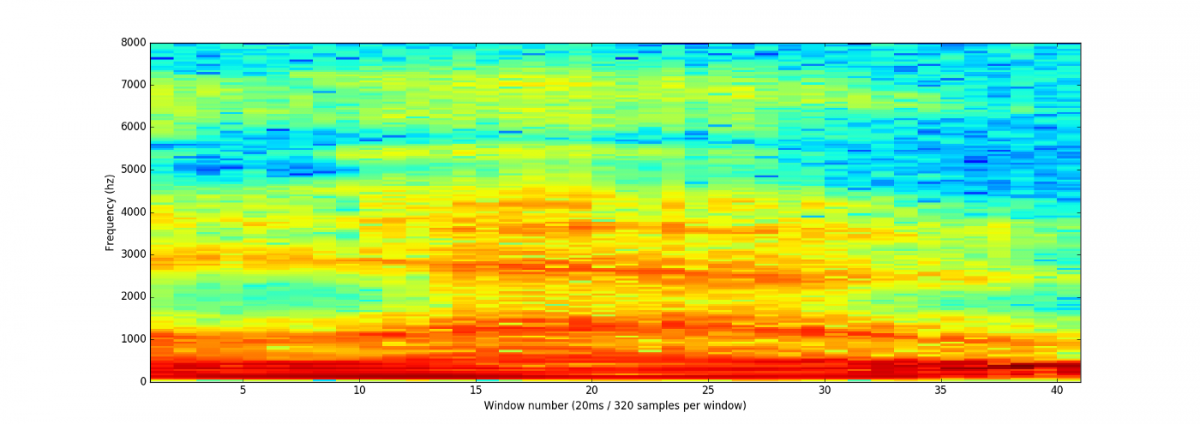
\includegraphics[width=0.7\linewidth]{img/spectogram}
    \caption{een voorbeeld van een spectrogram. \autocite{Vervoort2017}}
    \label{fig:spectrogram}
\end{figure}
Dit is het moment waar het neurale netwerk zijn werk begint te doen. Hij gaat aan elk stukje data een spraakklank toekennen. Spraakklanken zijn de klanken die samen een taal vormt. Voor de Nederlandse taal bestaan er 40 verschillende spraakklanken. Klanken worden in woordenboeken fonetisch beschreven om duidelijk te maken hoe woorden worden uitgesproken. Het neurale netwerk gaat uit een fonetische lijst de spraakklank halen die de grootste waarschijnlijkheid heeft om correct bij een audiosignaal te horen. Je kunt nooit helemaal zeker zijn dat er een bepaalde klank is uitgesproken. Dit klinkt eenvoudiger dan het is. Elke klank wordt namelijk door elke mens op een andere manier uitgesproken. Door het netwerk te trainen met een grote hoeveelheid data, zal het beter leren omgaan met deze verscheidenheid.

De laatste stap is het omzetten van de klanken naar woorden. De klanken worden aan elkaar gelinkt tot woorden. Ook hierbij helpt trainingsdata om accurater woorden en zinnen te vormen. Als het netwerk bijvoorbeeld twijfelt tussen de woorden hallo, aloo en haylow, dan zal het waarschijnlijkheid kiezen voor 'hallo' omdat dit waarschijnlijk vaker voorkomt in de trainingsset. Daarnaast houdt het ook rekening met de waarschijnlijkheid dat een bepaald woord volgt op een woord. Ter illustratie, een netwerk zal door te trainen begrijpen dat de kans groter is dat het woord 'voorbeeld' gevolgd is op woorden zoals 'als, een of goed' dan op woorden zoals 'inktvis of tafel'. Voor neurale netwerken populair werden werd hiervoor een andere techniek gebruikt, namelijk het Hidden Markov Model. Hoe dit model precies werkt is buiten de scope van dit onderzoek.
In deze uitleg werd de term neurale netwerken gebruikt. Het kan echter zijn dat anderen spreken over het toepassen van deep learning. Deep learning heeft er inderdaad voor gezorgd dat \gls{STT} geavanceerder werd. Eenvoudigweg is het een benaming voor complexe neurale netwerken. 

\subsection{Spraaksynthese}
Een andere techniek, die net het omgekeerde is van spraakherkenning, is spraaksynthese. Volgens ~\textcite{Rouse2016} is spraaksynthese menselijke spraak dat is gevormd door een computer. Spraaksynthese is de basis voor elk Text-To-Speech systeem. Het wordt gebruikt om geschreven tekst om te zetten naar gesproken taal, geproduceerd door de computer.
Spraaksynthese is aanwezig in ons dagelijkse leven. In automatische telefoongesprekken, de luchthaven, gps-systemen, op de bus en natuurlijk in digitale assistenten. \textcite{Seijas2018} vertelt dat er twee soorten methodes zijn voor Text-To-Speech. Concatenative , waar korte audiofragmenten aaneengeschakeld worde, is daar één van. Het is goed verstaanbaar omdat de woorden zijn opgenomen in hoge kwaliteit, maar het klinkt niet natuurlijk. Daarnaast is het ook veel werk om een grote databank te vullen met verschillende korte spraakfragmenten.\gls{TTS}
De andere methode, parametric \gls{TTS} is een meer statistische methode en  bedenkt de spraak gebaseerd op enkele parameters. Volgens \textcite{Oord2016} worden in die parameters de informatie opgeslagen die nodig is om gegevens te genereren. Parametric \gls{TTS} haalt taalkundige kenmerken uit de tekst. Bestaande parametrische modellen genereren typische audiosignalen door hun uitvoer door te geven via vocoders, algoritmen die signalen verwerken.

De grote opkomst van neurale netwerken heeft op de evolutie van spraaksynthese minder effect dan op de evolutie van spraakherkenning. De \gls{TTS} van vandaag is volgens \textcite{Oord2016} nog steeds grotendeels gebaseerd op concatenative \gls{TTS}. Deze methode klinkt ook nog steeds natuurlijker dan parametric \gls{TTS}, maar het is gemakkelijker om de stem aan te passen via parameters in het parametric model.

Een nieuwe doorbraak kwam er door het baanbrekende onderzoek van WaveNet. In \textcite{Singh2018} wordt verteld dat WaveNet een deep learning model is dat het mogelijk maakt om onbewerkte audiofragmenten te ontwikkelen o.b.v. directe geluidsopnames. Daarnaast is ook het aanpassen van de stem gemakkelijker geworden en klinkt het ook natuurlijker. Het wordt onder meer gebruikt door Google Assistant.
 
\subsection{Natural Language Processing}

Spraakherkenning en spraaksynthese zijn nodig in het ontwikkelen van een Voice User Interface (VUI), of stemgestuurde gebruikersomgeving, waar de gebruiker de computer als het ware bedient met zijn stem in plaats van bijvoorbeeld een toetsenbord of aanrakingen. De computer moet gesproken taal van de gebruiker begrijpen (spraakherkenning) en moet een gepast antwoord teruggeven (spraaksynthese). Spraakassistenten zoals Alexa, Siri of Google Assistant zijn voorbeelden van VUI's.

Omdat een assistent de spraak kan omzetten naar tekst betekent dit nog niet dat hij begrijpt wat iemand heeft verteld. Assistenten worden ontwikkeld met Natural Language Processing. Het is een methode om ongestructureerde data gebaseerd op de natuurlijke taal te verwerken tot een vorm die de computer kan begrijpen. Het zorgt ervoor dat de betekenis of het doel wordt achterhaald van wat iemand zegt. \gls{NLP} valt onder de noemer van Artificiële Intelligentie en het maakt gebruik van deep learning modellen. Modellen die getraind zijn om patronen te gaan herkennen in de menselijke taal door grote hoeveelheden aan data van bijvoorbeeld conversaties en berichten door te nemen. In principe is het vergelijkbaar met hoe een kind de taal leert, namelijk door naar voorbeelden te luisteren. \autocite{Rouse2017}
Volgens \textcite{Garbade2018} kan \gls{NLP} voornamelijk onderverdeeld worden in twee niveaus, syntaxis en semantiek. Syntaxis is de grammatica van de tekst leren begrijpen. Het splitsen van zinnen of woorden en elk deel identificeren is één van de vele functies. Semantiek is de betekenis van de tekst leren begrijpen. Algoritmen worden gebruikt om bijvoorbeeld woorden te interpreteren en te classificeren als persoonsnaam of plaatsnaam.

\section{Spraakassistenten}
Een spraakassistent, ook wel een virtuele, persoonlijke of slimme assistent genoemd, voert taken uit via verbale instructies van een gebruiker. Het is vooral aanwezig in smartphones, maar het wordt ook geïntegreerd in smart speakers, auto's of wearables. Dit onderzoek vergelijkt twee van de meest prestigieuze assistenten, Google’s Assistant en Amazon’s Alexa. Daarnaast zijn ook Apple's Siri, Microsoft's Cortana en Samsung's Bixby bekende voorbeelden.

\subsection{De geschiedenis van spraakassistenten}
\label{s:de geschiedenis van spraakassistenten}
De slimme spraakassistenten zijn vandaag gekend bij het grote publiek. Ze zijn ingebouwd in onze smartphones en slimme luidsprekers. Steeds paraat om ons de vertragingen te melden op de weg, het weer te voorspellen voor morgen of onze favoriete muziek te spelen. Het is iets van deze tijd, maar toch hebben ze al een lang pad van tientallen jaren bewandeld. Dit is hoe het allemaal begon en hoe we zijn geëvolueerd naar de bekende assistenten van vandaag.

\subsubsection{Jaren 50 - 60}
De eerste systemen die ietwat leken op een spraakassistent waren gefocust op het louter herkennen van de menselijke spraak. In \textcite{Vox-Creative2019} wordt geschreven hoe in  de Bell Laboratories in 1952 het ``Audrey'' systeem werd ontwikkeld. Audrey begreep de getallen 0 tot 9 op voorwaarde dat de sprekers tussen elk getal een pauze lieten. In theorie kon het gebruikt worden om met de stem een telefoonnummer in te geven. Onder andere de kost en omvang van de machine was groot. Het intoetsen van de telefoonknoppen bleef efficiënter, dus het effectieve gebruik van Audrey bleef uit.

\textcite{IBM2011} onthulde in 1962 de ``Shoebox'', een machine die met spraakcommando's eenvoudige berekeningen kon uitvoeren. De uitvinder William C. Dersch demonstreerde voor televisie hoe het apparaat, zo groot als een schoendoos, naast de getallen 0 tot 9 ook zes woorden zoals plus en totaal kon herkennen.

\begin{figure}[h]
    \centering
    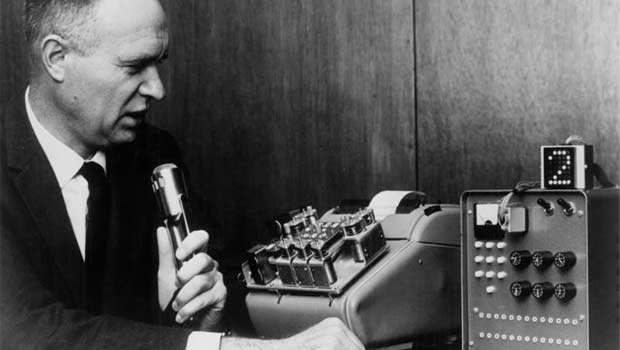
\includegraphics[width=0.7\linewidth]{img/Shoebox}
    \caption{William C. Dersch’s Shoebox deed eenvoudige berekeningen met spraakcommando's. \autocite{IBM2011}}
    \label{fig:shoebox}
\end{figure}

\subsubsection{Jaren 70 - 80}
Spraakherkenning in de jaren 70 werd vooral gekenmerkt door het departement voor defensie in de Verenigde Staten. Uit interesse voor spraakherkenning financierden ze een vijfjarig project over het thema. Volgens \textcite{Pinola2011} en \textcite{Kincaid2018} heeft dit geleid tot de ontwikkeling van Harpy in 1976. Harpy begreep 1011 woorden en kreeg vooral betekenis door haar efficiëntere zoekmethode, de ``Beam-search'', om logische zinnen te gaan herkennen.

In \textcite{Pinola2011} staat dat in de jaren 80 er een grote doorbraak kwam door de ontwikkeling van het hidden Markov model. Dit model gebruikt statistieken om een woord te herkennen in een onbekend geluid. Dit werd gedaan door het berekenen van de waarschijnlijkheid dat het onbekend geluid staat voor een bepaald woord. De woordenschat van de spraakherkenningssoftware bleef groeien tot een paar duizend woorden en had dankzij onder andere het hidden Markov model het potentieel om ongelimiteerd woorden te gaan herkennen.
Onder andere dankzij deze ontwikkelingen bleven ook de commerciële toepassingen niet uit. In 1987 kwam de Worlds of Wonder's doll Julie uit. Kinderen konden de pop trainen om te reageren op hun uitspraken. Dit staat zo beschreven in \textcite{Pinola2011}, waar je ook een reclamespot voor de pop kan bekijken. De technologie groeide snel, maar had wel een grote zwakte. De zin moest gedicteerd worden. Na elk woord werd dus een korte pauze verwacht.

\subsubsection{Jaren 90}
Volgens \textcite{Kincaid2018} kwam in de 90's automatische spraakherkenning in een eerste vorm zoals we het vandaag kennen. De doorbraak in die tijd heette Dragon. De eerste versie werd gelanceerd in 1990 onder de naam Dragon Dictate en had een woordenschat van 80 000 woorden. Daarnaast kon het iets nieuws, iets wat in de huidige spraakassistenten nog steeds gebruikt wordt, natural language processing. Zinnen moesten niet meer gedicteerd worden, maar Dragon kon oorspronkelijk 30 tot 40 woorden per minuut herkennen.

Volgens \textcite{Puri1998} is Dragon verantwoordelijk voor een doorbraak in spraakherkenningssoftware. De opvolger van de Dragon Dictate, Dragon NaturallySpeaking laat gebruikers spreken in een microfoon, aangesloten op de computer, en laat de woorden direct verschijnen op het computerscherm. Indien het een fout maakte, kon je het zelf corrigeren en kon de software leren uit zijn fouten. Het was ook de eerste spraakherkenningssoftware die toeliet om op een normale manier te praten.

\subsubsection{Van 2010 tot nu}
In \textcite{IBM2011} is te lezen hoe een mijlpaal werd bereikt door de Watson machine die won in Jeopardy. Watson was zo goed in taalverwerking dat hij 2 kampioenen in Jeopardy heeft verslaan live op televisie. Jeopardy is een Amerikaans spelprogramma waar de kandidaten het antwoord kregen en ze zelf de bijpassende vraag moesten geven. Watson was niet alleen goed in het samenstellen van correcte vragen, maar kon die ook telkens hardop uitspreken.

\begin{figure}[h]
    \centering
    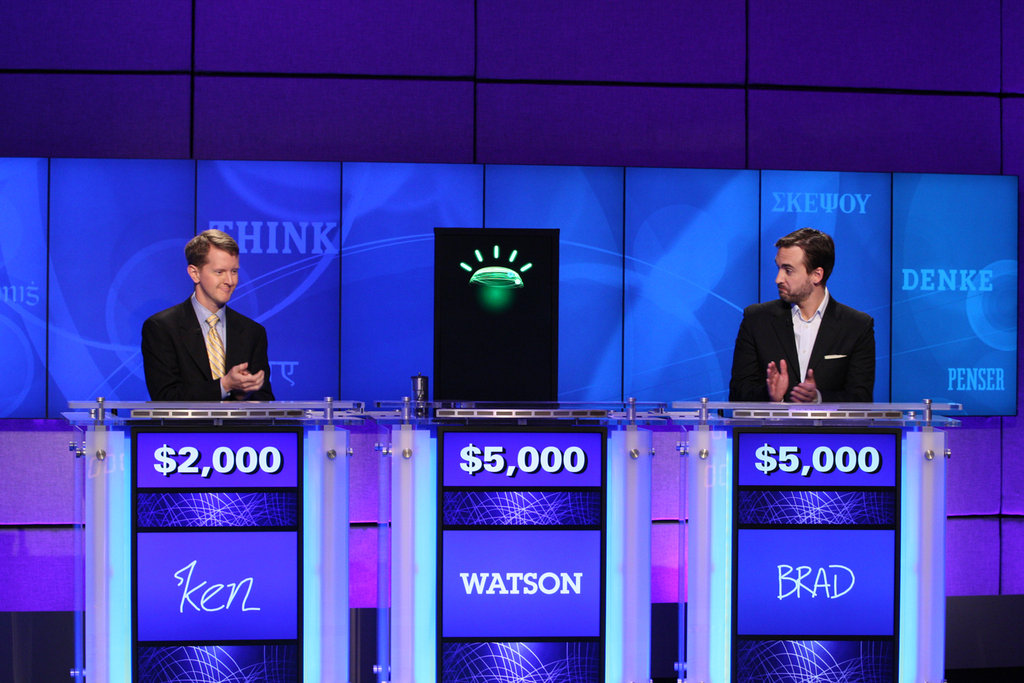
\includegraphics[width=0.7\linewidth]{img/WatsonJeopardy}
    \caption{Watson versloeg twee kampioenen in Jeopardy live op televisie. \autocite{Markoff2011}}
    \label{fig:watson}
\end{figure}

\subsection{De spraakassistenten van nu}
\label{ss:de spraakassistenten van nu}
Kort na deze gebeurtenis in 2011 werd Siri gebouwd in de Iphone 4S en werd zo de eerste spraakassistent voor het grote publiek uitgebracht. Siri is Apple's variant op de slimme spraakassistent en is tegenwoordig beschikbaar op meerdere apparaten met een IOS-besturingssysteem. Het grootste aandeel van de gebruikers kent Siri van op zijn Iphone, maar daarnaast is de assistent ook geïntegreerd in de Mac computer, de Apple Watch of de Apple TV. Ondertussen heeft het ook zijn eigen Smart Speaker, de HomePod. Siri is beschikbaar in het Nederlands.

Google gaf hierop een antwoord in 2012 door Google Now uit te brengen, de voorloper van de Google Assistant van vandaag. Volgens Google is de Google Assistant jouw eigen persoonlijke Google, die altijd bereid is om je te helpen wanneer je maar wilt. De Google Assistant bestond eerst onder de naam Google Now en was aanwezig in smartphones met een Android besturingssysteem. De Google Assistant van vandaag is te vinden in veel meer omgevingen. Smartphones, auto's, laptops, tablets, tv's, smartwatches en in hun eigen smart speaker, de Google Home. Deze speaker heeft ook een variant gekregen met een scherm, de Smart Display. Het is de enige assistant, op Siri na, die momenteel Nederlands begrijpt en spreekt.

Tijdens de Microsoft BUILD conferentie in 2013 werd Cortana geïntroduceerd als de spraakassistent van Microsoft. Cortana is ontwikkeld voor onder andere Windows 10, Windows Phone, Xbox One en in de slimme speaker Invoke.

In 2015 kwam de eerste slimme luidspreker op de markt. De Echo van Amazon, voorzien met hun slimme spraakassistent, Alexa. Amazon is één van 's werelds grootste bedrijven in het online verkopen van goederen. Het grote verschil met Google is dat de assistent voor het eerst werd gebruikt in de Echo, Amazon's smart speaker. Een groot nadeel aan Alexa is dat het vooral focust op de Amerikaanse markt en dus ook geen Nederlands kan. Amazon focust met Alexa vooral op de verkoop van artikelen via zijn gigantische online webshop. In de podcast van \textcite{Belghmidi2019a} vertelt e-commerce specialist Steven Van Belleghem dat 1 op 3 Amerikanen artikelen koopt door het te vragen aan Alexa.

\textcite{Lopez2018} besprak verschillende functionaliteiten van spraakassistenten Google Assistant, Alexa en Siri, op correctheid en natuurlijkheid bij 8 ondervraagden. In de administratieve categorie, zoals agendabeheer, to-dolijsten en alarmen kwam de Google Assistant als minst correct en minst natuurlijke assistent uit de bus, maar prijkt in de veelzijdige categorie (nieuws, weer, verkeer, woordbetekenissen, rekenen, enz.) dan weer ver bovenaan op beide vlakken. Algemeen werd de Google Assistant als de meest natuurlijke ervaren, onder andere door de toon van de stem die verwondering, onzekerheid en vreugde uitte.

Voor \textcite{Tulshan2019} stelden 100 personen allerlei vragen aan voice assistants Google Assistant, Alexa, Siri en Cortana. Ze gaven telkens een score op spraakherkenning en contextueel inzicht. Google Assistant kwam als grote winnaar uit het onderzoek door 59,80 \% van de vragen te beantwoorden. Een verschil van 15,82 \% met Siri, die de op één na nauwkeurigste bleek in dit onderzoek. Google Assistant was vooral leider in categoriëen als reizen, mailing, navigatie, vertalingen en begreep volgens het onderzoek goed de verschillende variaties in de stemmen van de onderzochte personen.

Volgens \textcite{Lopez2018} is de Echo Dot de favoriete smart speaker als het aankomt op het aankopen van artikelen. Dit is geen verrassing omdat hij oorspronkelijk ontworpen is om te winkelen en zelfs de enige spraakassistent is waarmee je online kan shoppen. In \textcite{Tulshan2019} bleek Alexa de minst nauwkeurige assistent te zijn met 7,91 \% nauwkeurigheid.

Slimme spraakassistenten worden alleen maar slimmer. \textcite{Brandt2018} heeft onderzocht hoe hoog het intelligentieniveau is van 4 slimme assistenten, namelijk Google Assistant, Microsoft Cortana, Amazon Alexa en Apple Siri in 2017 en 2018. De geanalyseerde gegevens zijn de antwoorden van de assistenten op 5000 algemene vragen. De beste prestatie werd verricht door Google Assistant die op 77,2 procent van de vragen een antwoord kon bieden, waarvan 95 procent correct. Bij alle assistenten zie je een verhoging van de intelligentie in vergelijking met het vorige jaar.

\begin{figure}[h]
    \centering
    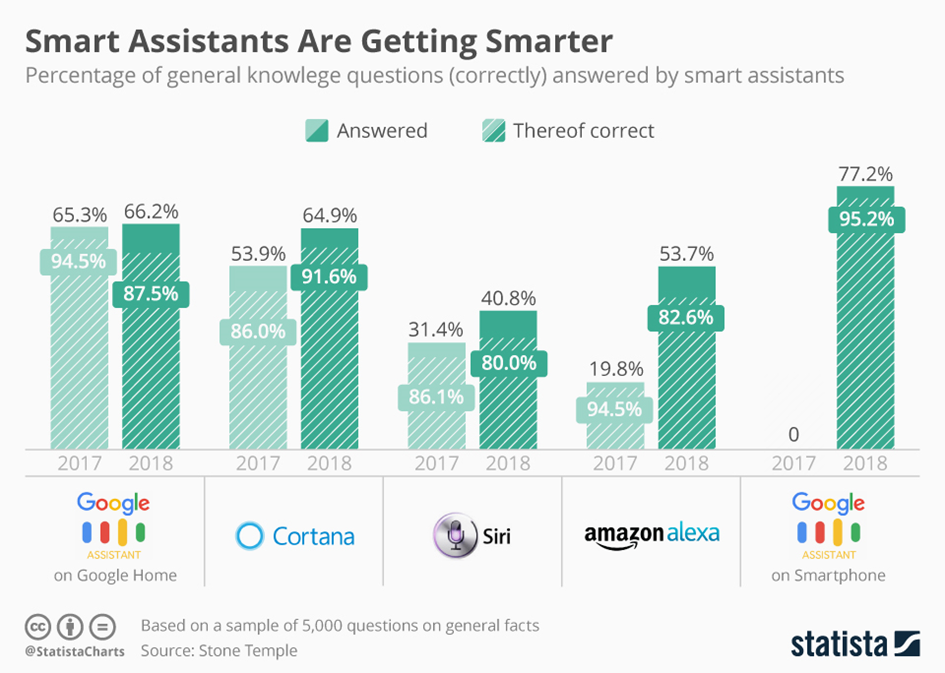
\includegraphics[width=0.7\linewidth]{img/SmartAssistantsAreGettingSmarter}
    \caption{Hoe hoog ligt het intelligentieniveau bij slimme spraakassistenten. \autocite{Brandt2018}}
    \label{fig:smartassistantsaregettingsmarter}
\end{figure}

Google spendeert veel middelen aan zijn assistent. Het heeft indruk gemaakt tijdens de recente Google I/O conferentie van dinsdag 7 mei 2019, waar ze onverwachts nieuws brachten. De volgende versie van de Google Assistant zal namelijk opvallend veel sneller gaan omdat ze de \gls{AI}-modellen die verantwoordelijk zijn voor \gls{NLP} offline beschikbaar hebben gemaakt. Dat wilt zeggen dat een commando van een gebruiker niet meer helemaal naar een server in Amerika moet transporteren om ervoor te zorgen dat de assistent het kan begrijpen. Vanaf de volgende versie zal deze logica afgehandeld worden door uw toestel zelf, omdat Google erin geslaagd is het geheugen van die modellen zo te reduceren dat het kan opgeslagen worden op uw apparaat. Het belooft dus dat binnenkort de gebruiker na het stellen van een vraag amper nog zal moeten wachten op een antwoord.

In een podcast van \textcite{Belghmidi2019a} wordt door specialist e-commerce Steven Van Belleghem voorspeld dat met een jaar 10 tot 15 procent van de Vlaamse gezinnen een slimme smart speaker in huis zullen hebben. Tegen dan zal het beschikbaar zijn op de Vlaamse markt en zullen er meer mogelijkheden bestaan. Hij voorspelt dat het net als de smartphone eerst een snufje wordt waar de early adapters mee willen pronken. De interfaces waar we mee communiceren zal veranderen. Persoonlijke digitale assistenten zullen overal aanwezig zijn om ons te helpen en zal een persoonlijk dienstverlening zijn om te helpen met alle zaken waar we geen tijd in willen stoppen.
Een grote reden waarom het op dit moment nog niet is ingeburgerd, is omdat er nog niet zo veel toepassingen zijn. Je kunt er voorlopig in België nog niet veel mee doen.

De voorspelling van Steven Van Belleghem wordt direct bekrachtigd door een nieuwsbericht op 28 mei. VRT NWS meldt dat de Belgische variant van de Google Assistant wordt uitgebracht. \autocite{Belghmidi2019} Voorlopig nog alleen met een Nederlands accent. Wat er wel bijkomt is de samenwerking met verschillende Belgische bedrijven. Zo kan iedereen binnenkort via de Google Assistant naar het radionieuws van VRT NWS luisteren, aan de NMBS vragen wanneer de volgende trein komt of artikelen van de Colruyt toevoegen aan zijn lijstje. Met deze aankondiging geeft Google het signaal dat ze de eerste intrede met een slimme spraakassistent wilt maken in België voor het grote publiek.

\section{Bestaande eerste hulpapplicaties}
\subsection{De Vlaamse EHBO-app van het Rode Kruis}
\label{ss:de vlaamse ehbo-app van het rode kruis}
Op 2 april ’19 kwam het Rode Kruis met het nieuws dat ze een app hebben ontwikkeld die kan helpen bij het geven van eerste hulp bij ongevallen. 80 procent van de Vlamingen weet niet wat hij moet doen als een nabije persoon begint te stikken, een hartstilstand krijgt of hevig begint te bloeden. Uit angst om iets fouts te doen, gebeurt er dan ook vaak niks. Met de app willen ze zoveel mogelijk mensen in staat stellen om hulp te verlenen. \autocite{Decroubele2019}

Het Rode Kruis benadrukt dat de applicatie de opleiding niet kan vervangen, maar dat het hulp kan bieden bij het geven van eerste hulp.

In de applicatie zijn er drie grote onderdelen, eerste hulp verlenen, eerste hulp leren en een \gls{AED}-toestel vinden in de buurt. Er zijn ook nog enkele opties die je naar de website van het Rode Kruis brengen om informatie te verkrijgen over het geven van bloed of plasma, het doen van een gift, het volgen van een opleiding of het aanmelden als vrijwilliger.

Als je eerste hulp wilt verlenen kun je uit het overzicht een onderwerp over eerste hulp kiezen, waarna je informatie krijgt over wat je moet vaststellen en wat je nodig hebt. Daarnaast geeft de app ook een stappenplan van instructies wat je moet doen. De levensbedreigende situaties staan helemaal bovenaan en zijn voorzien van extra ingesproken instructies.

Als je eerste hulp wilt leren kun je eerst een onderwerp kiezen. Voorbeelden zijn een beroerte of alcoholvergiftiging. Daarna krijg je over het onderwerp vragen \& antwoorden, informatieteksten en video's. Per leerdeel krijg je een quiz die je moet oplossen om bepaalde badges te verdienen.

Wanneer iemand in uw omgeving een hartstilstand krijgt dan kun je met de applicatie een kaart openen waar \gls{AED}-toestellen staan op gesitueerd. Je kunt er ook een nieuwe \gls{AED} melden of meer informatie lezen. Met een \gls{AED}-toestel kan je defibrilleren. Het doet het hart stilstaan, zodat de normale hartmechanismen de controle opnieuw kunnen overnemen. \autocite{Gezondheidbe2018} Volgens \textcite{Koster1999} heeft het belang van vroegtijdig defibrilleren voor het verhogen van de overlevingskans geleid tot het concept van de ‘eerste hulp’-defibrillatie en het \gls{AED} toestel. Tegenwoordig zijn er in België \gls{AED}’s voorzien op verschillende openbare plaatsen zoals sporthallen, scholen of grote bedrijven om er voor zorgen dat defibrillatie vroegtijdig kan uitgevoerd worden door niet-medisch personeel, in afwachting van de komst van getraind medisch personeel.

\subsection{De Nederlandse EHBO-app van het Rode Kruis}
Nederland heeft al langer een mobiele EHBO-applicatie. Deze verschilt niet zo veel met de Belgische versie. Ze heeft wel een zoekfunctie om sneller de instructies voor uw ongeval te vinden. Je kan er ook EHBO-kits en cursussen bestellen in de webshop.
%%=============================================================================
%% Methodologie
%%=============================================================================

\chapter{Methodologie}
\label{ch:methodologie}

\section{De keuze van de spraakassistenten}
Er is een reden waarom Siri niet mee wordt opgenomen in dit onderzoek. Ondanks dat het Nederlands ondersteunt is het toch geen goede optie voor dit onderzoek omdat je beperkt bent in het ontwikkelen van een eigen applicatie. Apple werkt met Sirikit, een framework die je alleen kan gebruiken om Siri te verwerken in je eigen IOS-applicatie. Je kunt dus geen eigen voice-applicatie maken van scratch, maar je bent verplicht om te vertrekken vanuit een mobiele applicatie. Je kunt dus alleen een bestaande applicatie uitbreiden met een optie om aan Siri vragen te stellen die hiermee te maken hebben.

Daarnaast heb je ook nog eens de beperking dat Siri alleen kan gebruikt worden op een Apple device. Binnen het kader van dit onderzoek is het belangrijk om te testen met hetzelfde apparaat. Er moet zoveel mogelijk gewerkt worden in weinig veranderlijke omstandigheden. Om te vermijden dat de hardware een invloed heeft op de resultaten worden de assistenten gebruikt op hetzelfde toestel. Sommige resultaten kunnen namelijk afhangen van de smartphone zijn prestaties. Dezelfde beperking geldt voor Bixby, die enkel kan gebruikt worden op een smartphone van Samsung.

Er is ook gezocht naar open-source projecten. Zo bestaat er Mycroft. Het grote voordeel aan Mycroft is dat het, in tegenstelling tot Google Actions of Alexa Skills, niet gekoppeld is aan een enterprise. Het is volledig open en het kan gebruikt worden in allerlei toepassingen, van een wetenschappelijk onderzoek tot een softwareapplicatie voor een bedrijf. Je kunt de software van Mycroft zelf gaan veranderen, uitbreiden en verbeteren. Daarnaast kan je ook nog kiezen voor een apparaat waar je de Mycroft software op wilt draaien. Een gewone desktop, een auto of een Raspberry Pi zijn enkele van de mogelijkheden.
De software bestaat nog niet zo lang en helaas zijn mankementen al snel zichtbaar. Iets wat direct opvalt bij het opzetten van een Android project met Mycroft is dat de documentatie heel schaars is. Sommige stappen in de documentatie staan zelfs nog beschreven als to-do. Ze bieden wel een smart speaker aan, maar die wordt weinig verkocht.

Na eerder opgesomde redenen wordt beslist om enkel Amazon Alexa en Google Assistant verder te onderzoeken. Meer specifiek zal de Amerikaans-Engelse Alexa vergeleken worden met de Amerikaans-Engelse Google Assistant en de Nederlandstalige Google Assistant uit Nederland.

\section{Wat wordt er vergeleken}
\label{sec:vergelijking van stemgestuurde assistenten}
In het onderzoek worden de kwaliteit van spraaksynthese en de kwaliteit van spraakherkenning gemeten. Twee onmisbare functionaliteiten die de afgelopen jaren door neurale netwerken zo zijn verbeterd dat het mogelijk werd om op een aangename en natuurlijke manier met spraakassistenten te communiceren. Uitgebreide informatie over \gls{STT} en \gls{TTS} is beschreven in \ref{s:spraakgestuurde technologie}.

om de kwaliteit van de spraaksynthese te meten worden er vijf eigenschappen onderscheiden die hier aan meedragen. De gebruiker beoordeelt elke assistent na het beluisteren van drie antwoorden op deze eigenschappen. Deze zijn verstaanbaarheid, menselijkheid, levendigheid, tempo en emotionaliteit. Ze zijn gekozen met het oog op een EHBO-applicatie waar het belangrijk is dat de instructies goed worden verstaan. De gebruiker moet kunnen luisteren naar een stem die klinkt als een mens en niet als een robot. De instructies mogen niet te snel en niet te traag uitgesproken worden. De levendigheid en het gevoel die aanwezig zijn in de stem van de assistent zullen ook een positieve invloed hebben op de spraakkwaliteit. De deelnemers beoordelen deze eigenschappen met de likertschaal, waarbij een score wordt gegeven van 1 tot 5. Wie de details over deze eigenschappen en hoe ze worden beoordeeld wilt kennen, kan de vragenlijst inkijken waar naar wordt verwezen in \ref{ss:deel één: met de deelnemer}.

Om te vergelijken hoe goed de assistenten spraak kunnen omvormen naar tekst, wordt er gemeten hoe sterk een bepaalde vraag die een gebruiker heeft gesteld verschilt van de zin die de assistent er van heeft gemaakt. Die sterkte wordt uitgedrukt in aantal fouten. Een fout wordt gezien als een woord uit de originele vraag die niet is opgenomen in de gevormde zin van de assistent.

\section{Gebruikte materialen}
Voor het onderzoek zijn volgende zaken gebruikt:
\begin{itemize}
    \item Acer Aspire F 15 laptop
    \begin{itemize}
        \item Intel Core I5
        \item geïntegreerde microfoon
        \item 2,5 jaar in gebruik
    \end{itemize}
    \item Xiami Redmi note 4 smartphone
    \begin{itemize}
        \item Android 7.0
        \item Octa core processor
        \item 4 GB RAM
        \item 2 jaar in gebruik
    \end{itemize}
    \item Ultimate Ears BOOM 2 Speaker
    \begin{itemize}
        \item 12,5 watt vermogen
        \item 90dB gevoeligheid
        \item 3,5mm mini-jack (AUX) ingang
        \item 1,5 jaar in gebruik
    \end{itemize}
    \item 3.5mm Jack kabel
    \item Google Assistant app voor Android
    \item Alexa Beta app voor Android
\end{itemize}

\section{Het verloop van het onderzoek}
\subsection{Deel één: met de deelnemer}
\label{ss:deel één: met de deelnemer}
De steekproef bestaat uit 30 Vlamingen tussen 19 en 60 jaar die Nederlands spreken als moedertaal en enige kennis hebben van de Engelse taal. Het onderzoek is afgenomen in twee grote delen.

De onderzoeker volgt voor dit deel een vast stappenplan die te vinden is in de map onderzoek in de repository beschreven in \ref{s:verwijzing naar repository}.
De vragenlijst die tijdens dit deel wordt ingevuld is te vinden in de map bijlagen in de repository beschreven in \ref{s:verwijzing naar repository}.
Er is een kleine applicatie ontwikkeld voor elke assistent waar de gebruiker drie vaste EHBO-gerelateerde vragen kan stellen en telkens een vast antwoord terugkrijgt. De applicaties voor de Google Assistant zijn ontwikkeld met DialogFlow en de Actions-On-Google console. De applicatie voor Alexa is ontwikkeld in de Alexa Developer Console. Om de juiste antwoorden te voorzien is er ook code geschreven. Het project is te vinden in de map ehbo-app/testApp-ehbo-Alexa in de repository beschreven in \ref{s:verwijzing naar repository}.

\begin{figure}[H]
    \centering
    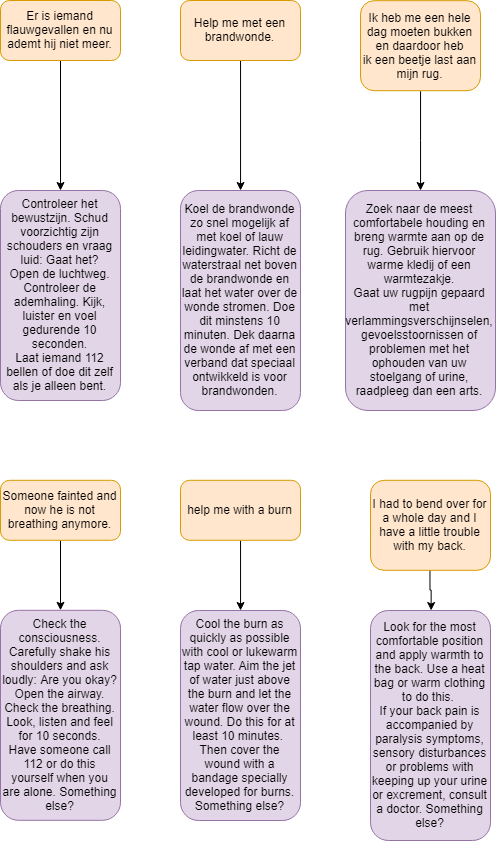
\includegraphics[width=0.7\linewidth]{img/flowdiagram_testapp}
    \caption{De flowchart waar de applicaties voor de test op zijn gebaseerd}
    \label{fig:flowdiagram}
\end{figure}

Voor het eerste deel stellen de deelnemers drie Engelse en drie Nederlandse EHBO-gerelateerde vragen aan een fictieve spraakassistent. De gestelde vragen worden opgenomen door een laptop.
Om te beginnen leest de deelnemer een korte introductietekst over spraakassistenten en vult hij enkele algemene vragen in. Daarna krijgt hij zes bladeren met op elk blad een vraag. Hij wordt aangespoord door de onderzoeker om elke vraag eerst in stilte te lezen om hem daarna te stellen aan de assistent. De aanwezigheid van een spraakassistent wordt geveinsd omdat de manier waarop de deelnemer de vragen stelt vergelijkbaar moet zijn aan de manier waarop hij ze zou stellen aan een echte assistent. De participant krijgt nooit een antwoord te horen, waardoor de mogelijkheid ontstaat dat hij steeds meer zijn best doet de volgende vraag duidelijker uit te spreken. Het verkregen resultaat zijn opgenomen audiofragmenten die later worden gebruikt in het tweede deel.

Na het stellen van alle vragen wordt de deelnemer op de hoogte gebracht van de assistent zijn afwezigheid en krijgt hij een volgende taak. Hij moet nu aan drie bestaande assistenten telkens dezelfde drie vragen stellen en te luisteren naar de drie antwoorden. Er wordt benadrukt dat het niet gaat om de inhoud van het antwoord, maar om de kwaliteit van de stem en de manier waarop het wordt gebracht. De participant krijgt de antwoorden van de assistent te horen door een speaker die met een kabel is aangesloten aan een smartphone. Hij kan de vragenlijst over de assistenten hun spraakkwaliteit al eens doornemen. De participant wordt door de onderzoeker aangespoord om goed te luisteren. Hij mag vragen opnieuw stellen tot hij antwoord krijgt van de assistent. Telkens nadat een assistent de drie vragen heeft beantwoord wordt de vragenlijst over die assistent ingevuld. De deelnemer krijgt na elke beoordeling de kans om vorige beoordelingen van assistenten aan te passen. Op het einde vult de participant nog enkele algemene vragen in.

\begin{figure}[h]
    \centering
    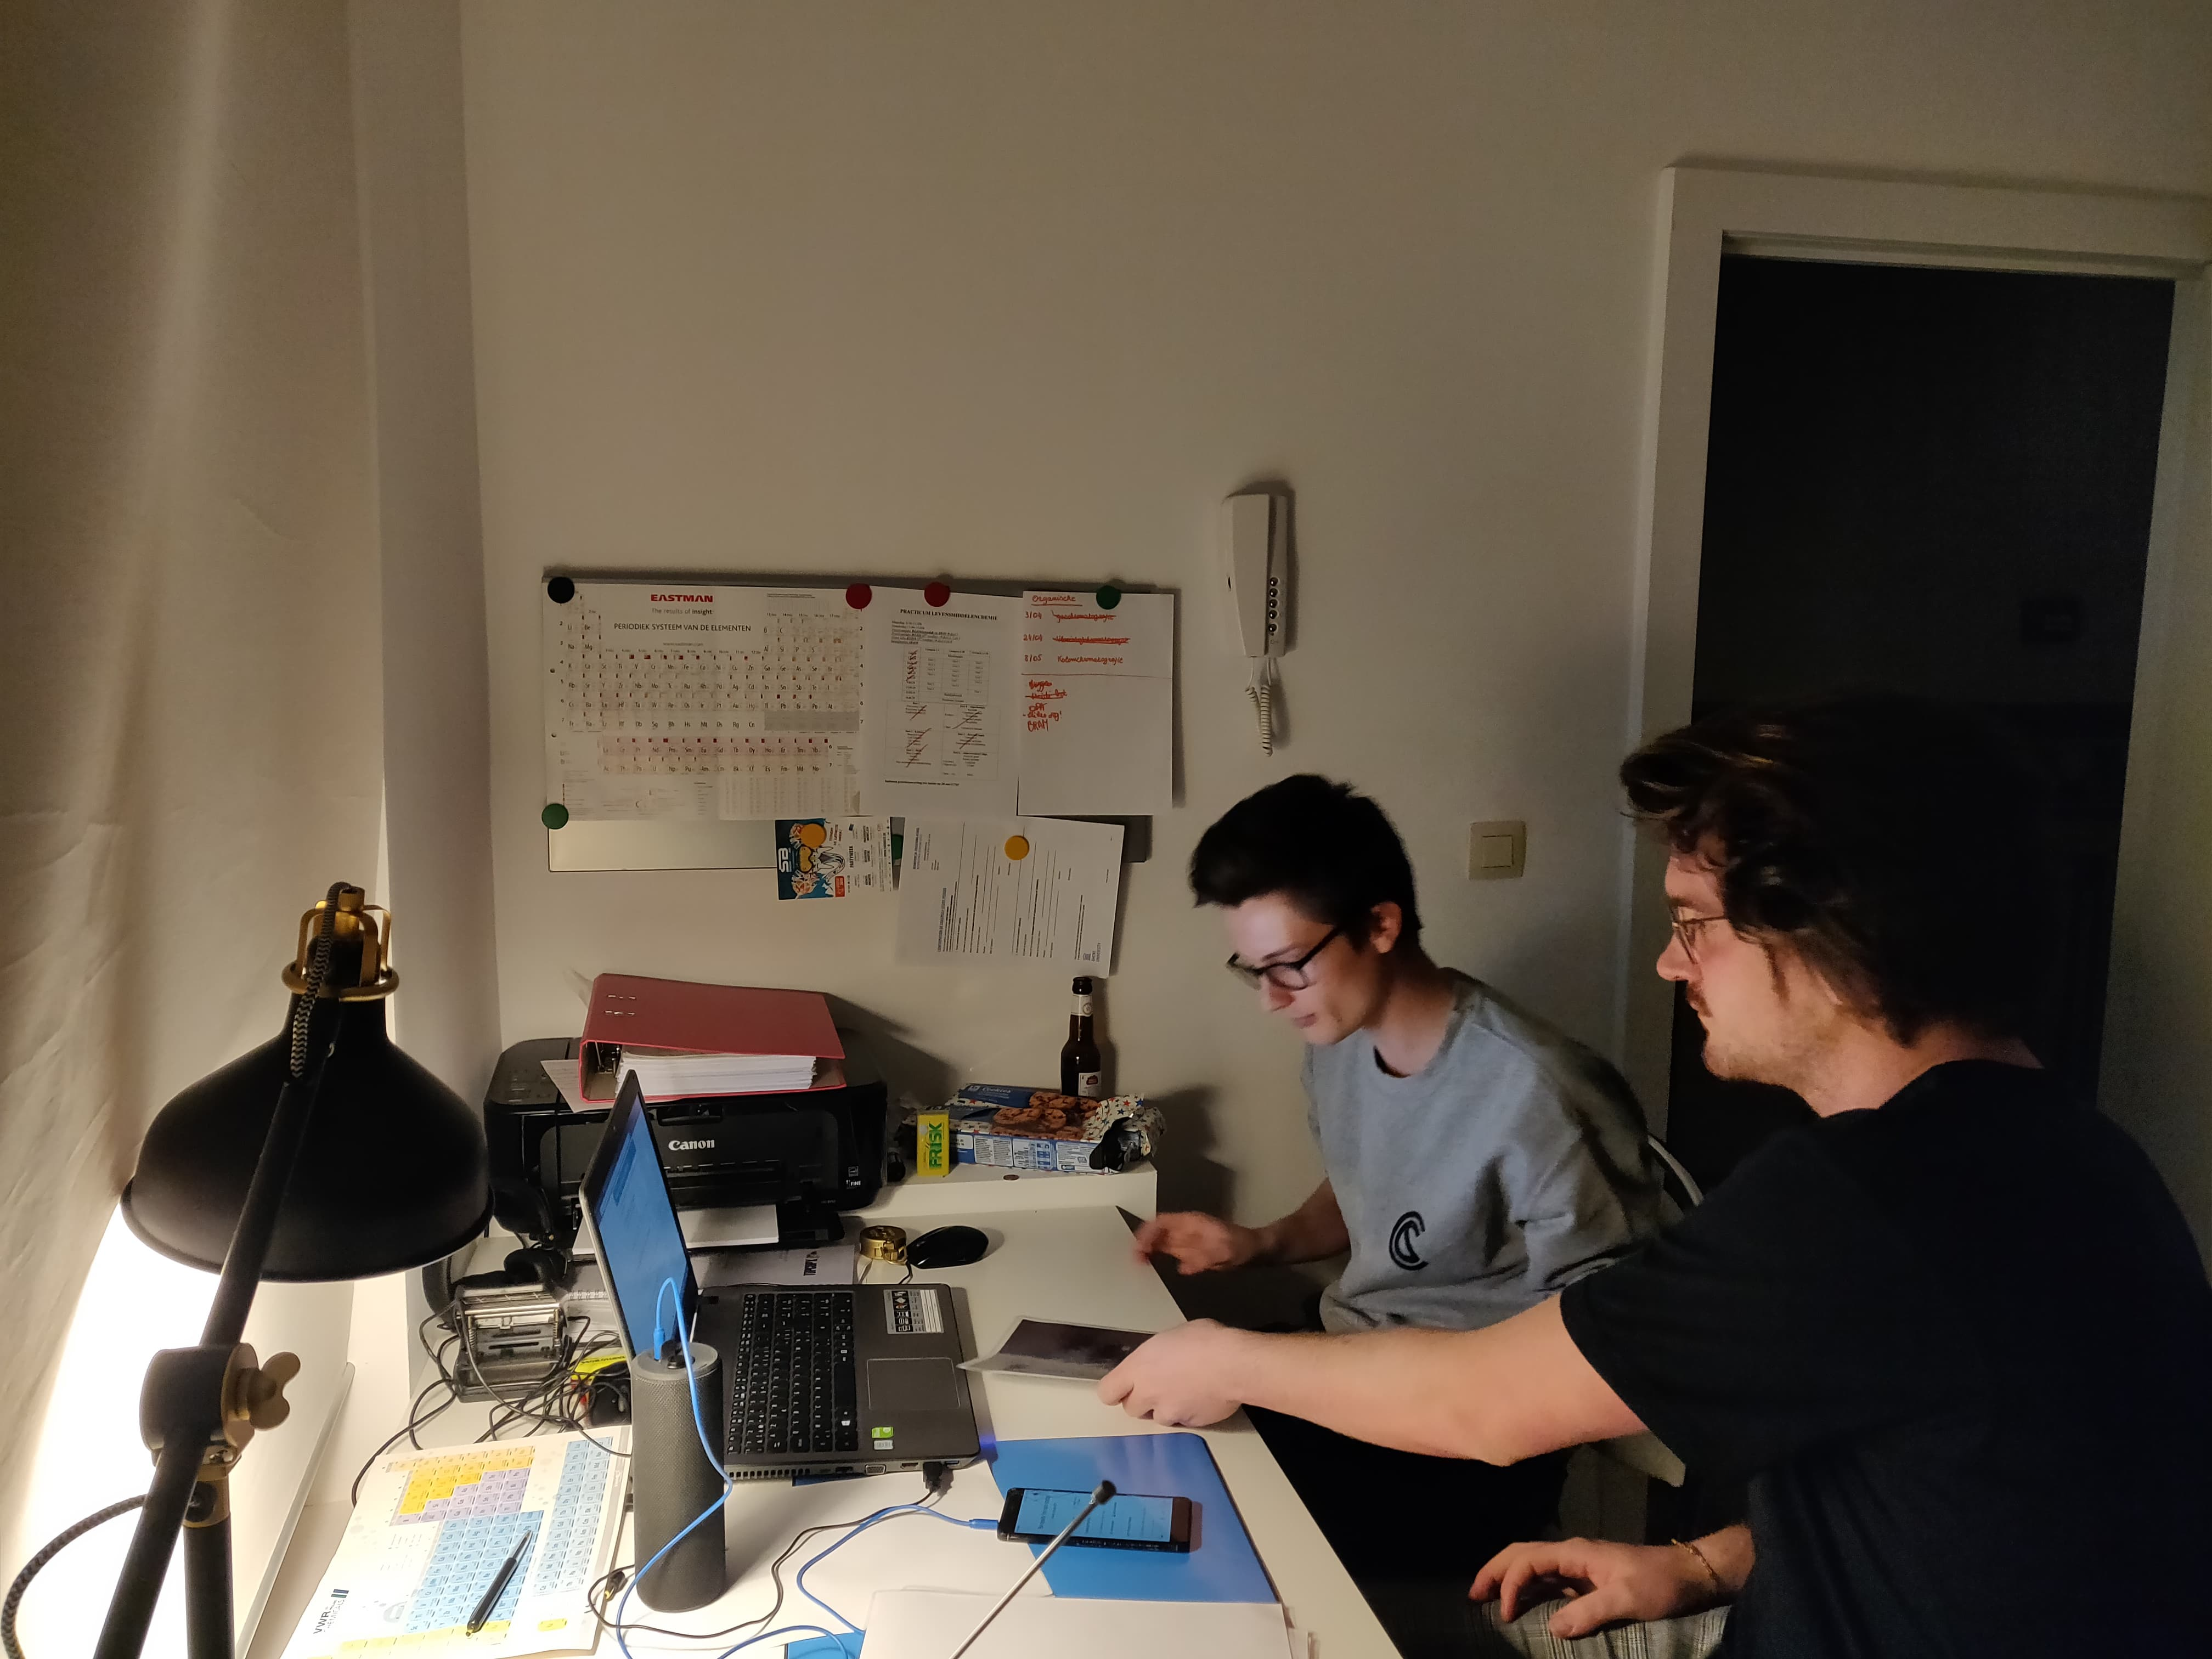
\includegraphics[width=0.7\linewidth]{img/proefafname2}
    \caption{Een deelnemer ontvangt de vragen die hij zal stellen aan de assistenten.}
    \label{fig:proefafname1}
\end{figure}

\subsection{Deel twee: zonder de deelnemer}
De vragenlijst die tijdens dit deel wordt ingevuld is te vinden onder de map bijlagen in de repository beschreven in \ref{s:verwijzing naar repository}.

Tijdens het tweede deel van het onderzoek luisteren de assistenten naar de vragen van de deelnemer. Er wordt gemeten hoe de assistenten deze vragen van spraak omzetten naar tekst. 
Er is beslist om de Nederlandse Google Assistant niet te betrekken in dit deel van het onderzoek. De reden hiervoor is dat de vragen anders zijn in het Nederlands en er figuurlijk appels zouden vergeleken worden met peren. Het aantal fouten vergelijken is niet mogelijk omdat de vertaalde vragen in het Nederlands een ander aantal woorden bevat dan de Engelse zinnen.

Er werden maatregelen genomen om de beïnvloeding van veranderlijke factoren te beperken. Zo werd tijdens het afnemen van het onderzoek beslist om de Nederlandse assistent hier niet meer bij te betrekken. De reden hiervoor was dat de Nederlandse assistent een Nederlandse vertaling van de zinnen moet herkennen, waardoor het aantal woorden in de zinnen verschillen van de Engelse zinnen. Hierdoor zou de vergelijking van het aantal fouten niet meer kloppen.

Een persoon zal ook nooit twee keer een vraag op exact dezelfde manier uitspreken. Als de deelnemer elke vraag al kan stellen zonder versprekingen dan nog zal er altijd een verschil zijn in onder meer volume, snelheid en intonatie. Daarnaast is er ook nog de extra beïnvloeding van externe ruis.
Een oplossing kan zijn om drie toestellen te gebruiken die elk voorzien zijn van een andere assistent. De gebruiker kan dan de vraag eenmalig stellen terwijl de drie assistenten tegelijkertijd luisteren. Ondanks dat dit op het eerste zicht een goede oplossing lijkt, zijn er toch enkele bedenkingen. Wegens financiële redenen is het voor de onderzoeker niet mogelijk om drie nieuwe smartphones aan te kopen. Moest dit toch mogelijk zijn dan kan er nog steeds een verschil van kwaliteit in de microfoon aanwezig zijn. Elk apparaat is uniek. Als er met drie gebruikte smartphones wordt gewerkt zal het verschil zeker aanwezig zijn door slijtage of ongelijk model.

Dit is de reden waarom de vragen zijn opgenomen in deel één. Een geregistreerd audiofragment maakt het mogelijk om de identieke vraag drie keren af te spelen terwijl telkens één assistent meeluistert op hetzelfde apparaat. Dit gebeurt in een geluidsdichte opnamestudio om externe ruis tijdens dit proces zoveel mogelijk te beperken. Er kan wel ruis mee opgenomen zijn tijdens deel één, of een deelnemer kan zich versproken hebben, maar die elementen zijn dan aanwezig bij elke assistent die het audiofragment hoort. De fragmenten worden afgespeeld door een speaker die aangesloten is op een laptop met een kabel.

\begin{figure}[H]
    \centering
    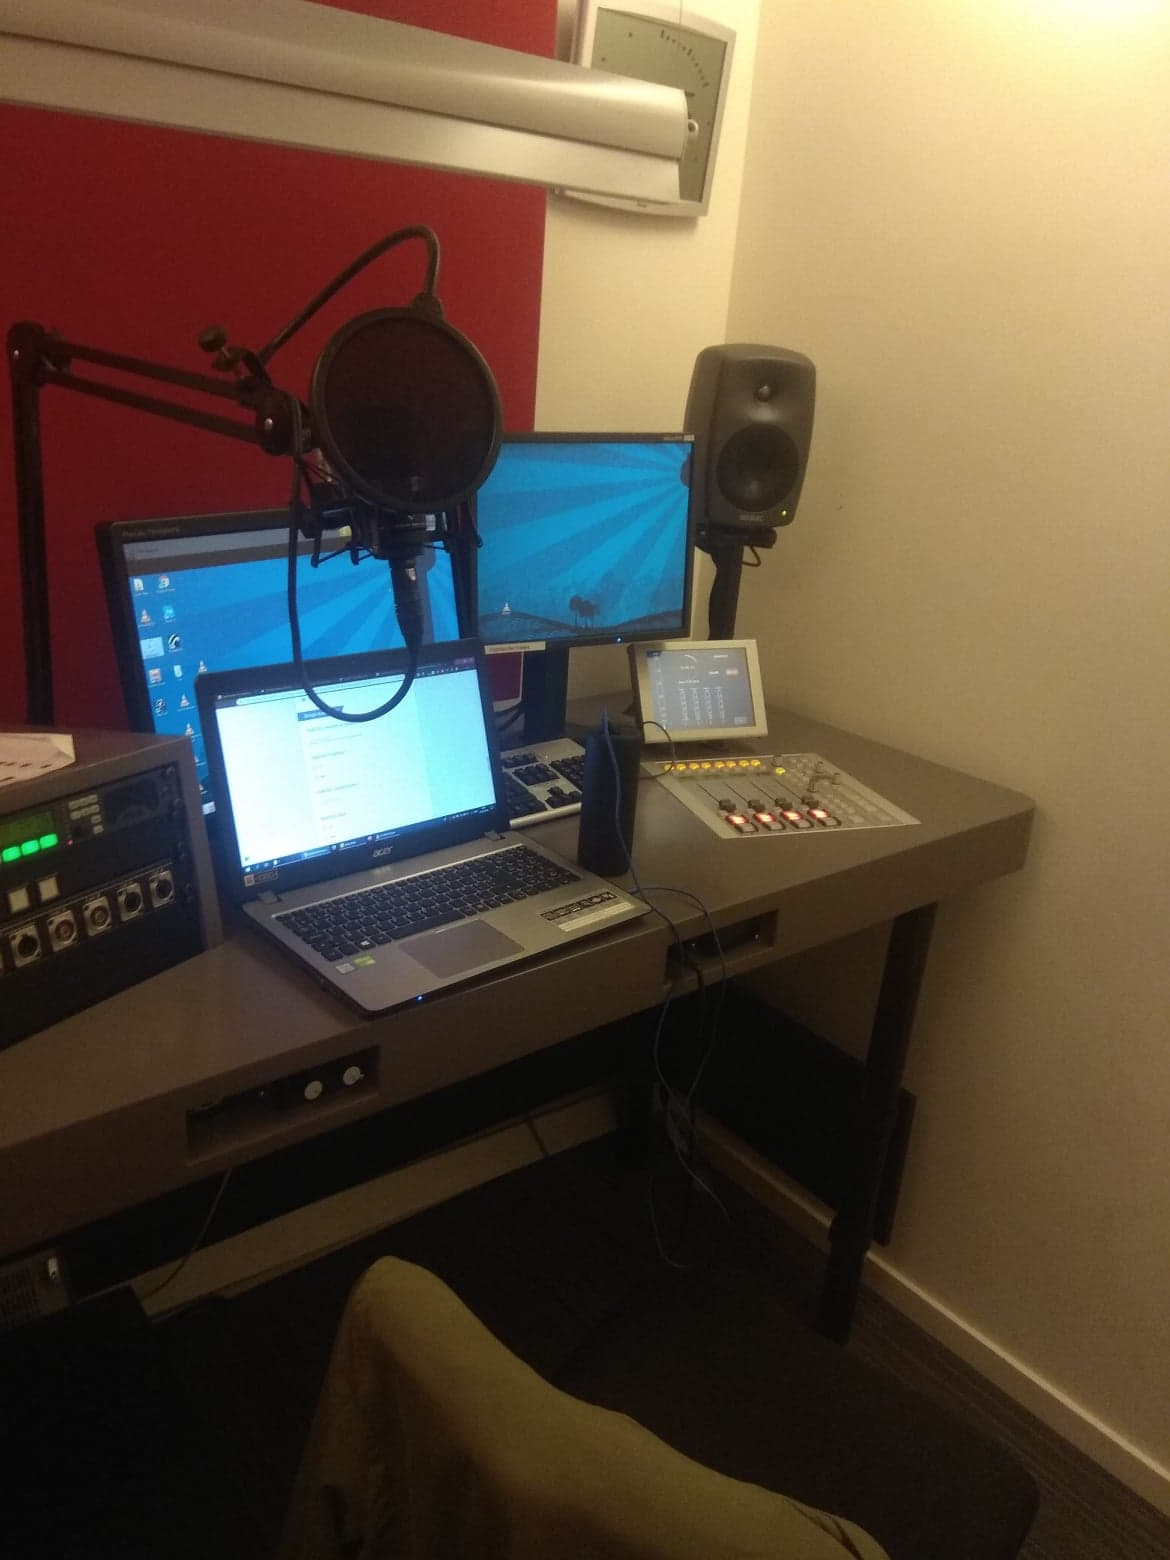
\includegraphics[width=0.7\linewidth]{img/proefafname3}
    \caption{De audiofragmenten worden beluisterd door de assistenten in een geluidsdichte studio.}
    \label{fig:proefafname2}
\end{figure}

Het is belangrijk om in achting te nemen dat de vragen niet zijn gesteld in de ontwikkelde applicaties uit deel één, maar direct aan de assistent zelf. Als je een applicatie ontwikkelt voor een spraakassistent dan verzamel je trainingszinnen zodat de applicatie weet op welke zinnen hij kan reageren. De ontwikkelaar kan uitgebreid trainingszinnen verzamelen om ervoor te zorgen dat de spraakherkenning verbeterd. Daarnaast toont Alexa in een applicatie niet altijd de rauwe tekst die hij herkent, maar soms de trainingszin die hij eraan koppelt. Het is gewoon niet duidelijk bij Alexa of hij de tekst toont die hij echt heeft begrepen of de trainingsvraag die hij er in herkent heeft. Misschien is Google wel even goed in het herkennen van een zin, maar toont Alexa direct de trainingsvraag in plaats van de tekst die hij heeft geïnterpreteerd. Om ervoor te zorgen dat de trainingszinnen geen invloed hebben op het resultaat, worden de vragen niet gesteld terwijl de applicatie is geopend. Ze worden aan de assistent zelf gesteld. Die moet het dan alleen doen met de ingebouwde speech-to-text functionaliteit en kan geen rekening houden met opgestelde trainingszinnen van de ontwikkelaar.

Zowel Alexa als Google Assistant maken het mogelijk om een overzicht van uw interacties te bekijken. Na de audiofragmenten van de 30 gebruikers af te spelen voor elke assistent werd dit overzicht gebruikt om de vragenlijst in te vullen. In de vragenlijst wordt de gevormde tekst van de assistent genoteerd samen met het aantal fouten die het bevat.
%%=============================================================================
%% resultaten vergelijkend onderzoek
%%=============================================================================

\chapter{Resultaten vergelijkend onderzoek}
\label{ch:resultaten}
Wie in detail wilt bekijken hoe de resultaten zijn bekomen, kan meer informatie vinden bij \ref{appendix:stappenplan analyse}.

\section{Vergelijking van de assistenten in spraakkwaliteit}
\label{s:Vergelijking van de assistenten in spraakkwaliteit}

\subsection{Vergelijking van de assistenten per eigenschap}
\label{ss:Vergelijking van de assistenten per eigenschap}

\begin{figure}[H]
    \centering
    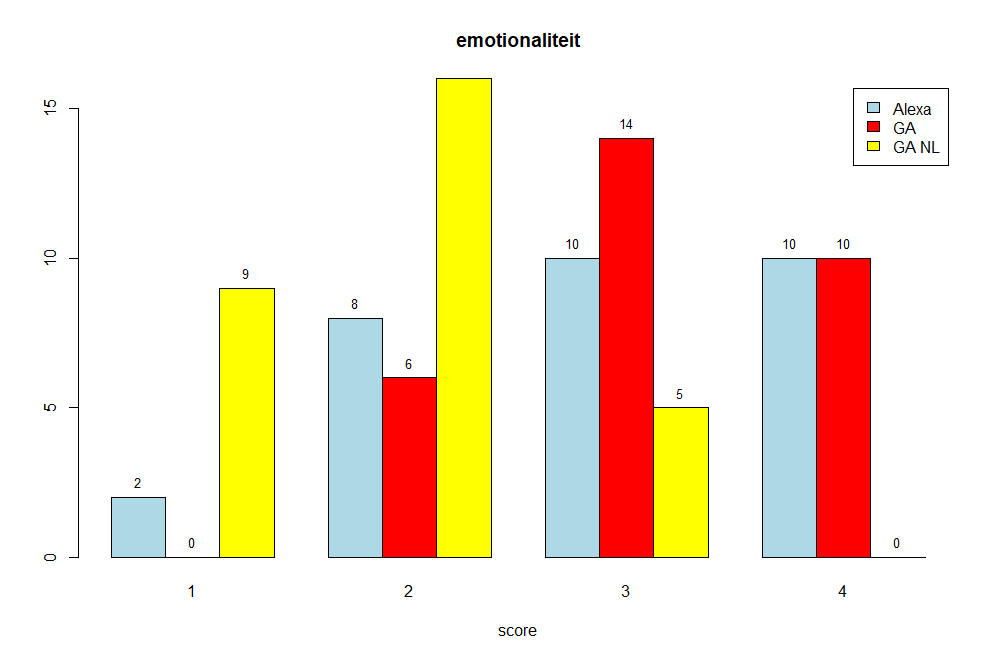
\includegraphics[width=0.9\linewidth]{../onderzoek/onderzoeksresultaten/vergelijking_assistenten_per_eigenschap/barplot/barplot_score_emotionaliteit}
    \caption{De scores die de deelnemers hebben gegeven op de emotionaliteit van de assistenten}
    \label{fig:barplot-emotionaliteit}
\end{figure}

\begin{figure}[H]
    \centering
    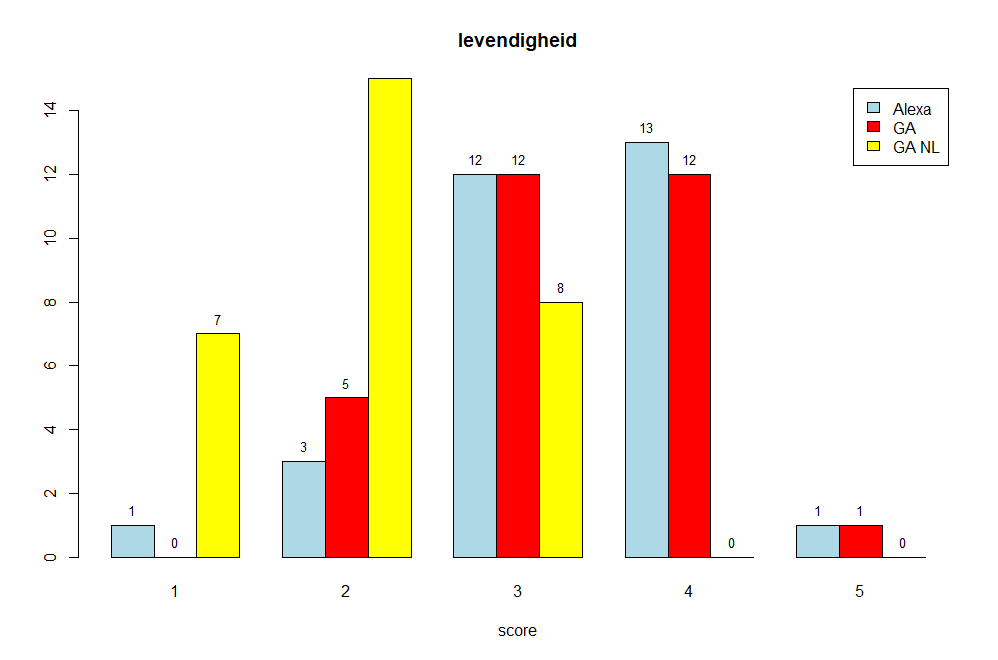
\includegraphics[width=0.9\linewidth]{../onderzoek/onderzoeksresultaten/vergelijking_assistenten_per_eigenschap/barplot/barplot_score_levendigheid}
    \caption{De scores die de deelnemers hebben gegeven op de levendigheid van de assistenten}
    \label{fig:barplot-levendigheid}
\end{figure}

\begin{figure}[H]
    \centering
    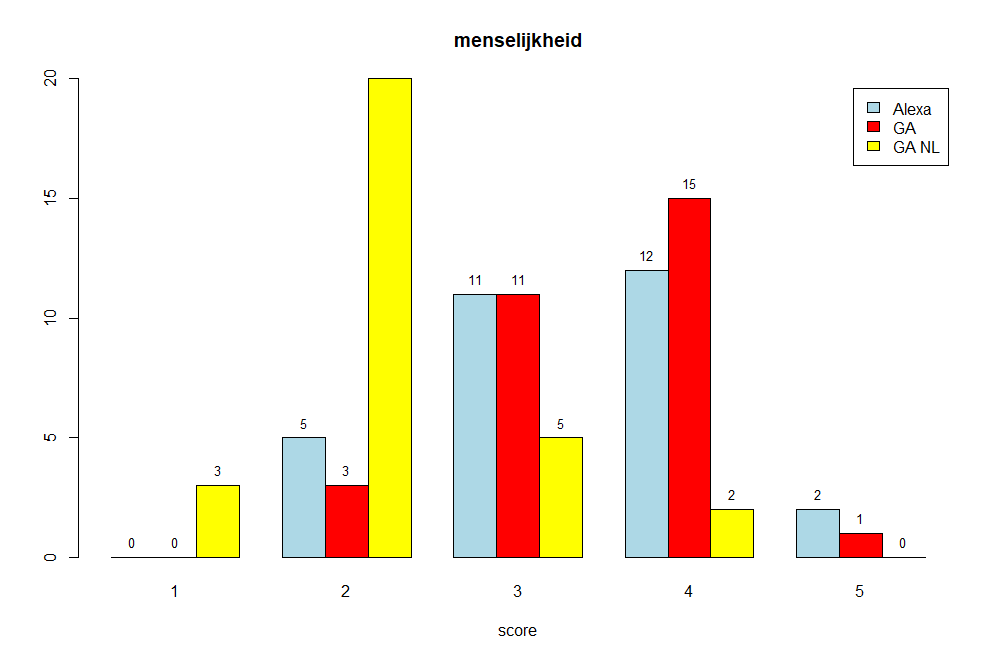
\includegraphics[width=0.9\linewidth]{../onderzoek/onderzoeksresultaten/vergelijking_assistenten_per_eigenschap/barplot/barplot_score_menselijkheid}
    \caption{De scores die de deelnemers hebben gegeven op de menselijkheid van de assistenten}
    \label{fig:barplot-menselijkheid}
\end{figure}

\begin{figure}[H]
    \centering
    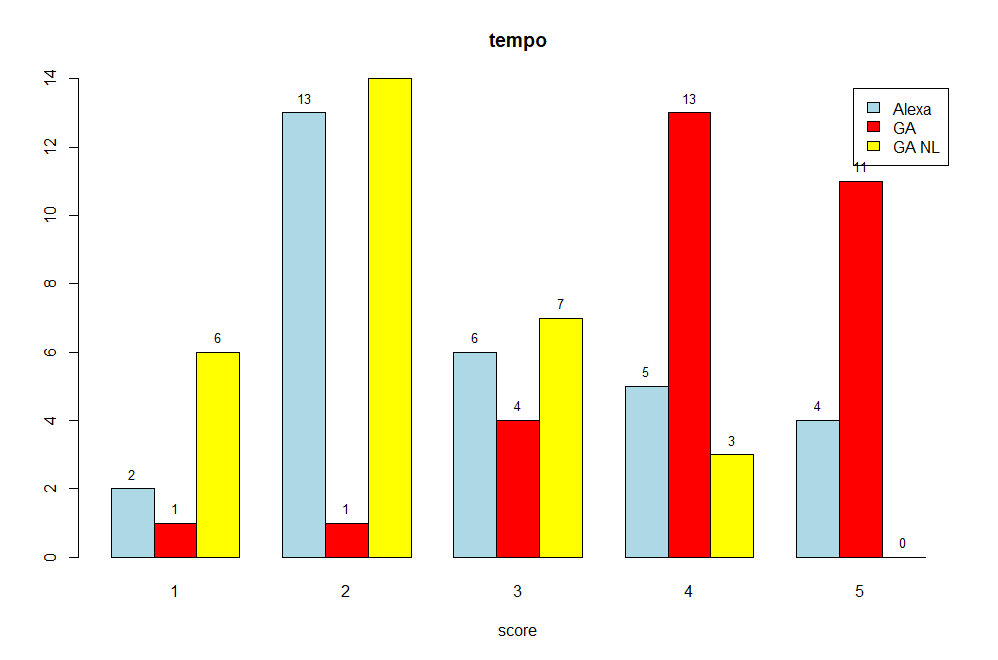
\includegraphics[width=0.9\linewidth]{../onderzoek/onderzoeksresultaten/vergelijking_assistenten_per_eigenschap/barplot/barplot_score_tempo}
    \caption{De scores die de deelnemers hebben gegeven op het tempo van de assistenten}
    \label{fig:barplot-tempo}
\end{figure}

\begin{figure}[H]
    \centering
    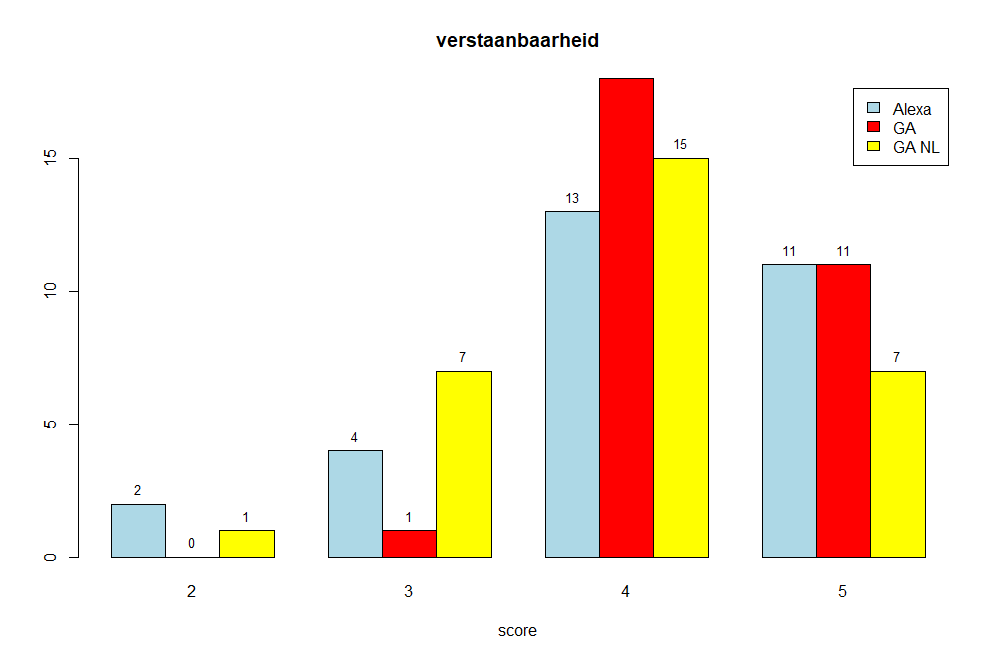
\includegraphics[width=0.9\linewidth]{../onderzoek/onderzoeksresultaten/vergelijking_assistenten_per_eigenschap/barplot/barplot_score_verstaanbaarheid}
    \caption{De scores die de deelnemers hebben gegeven op de verstaanbaarheid van de assistenten}
    \label{fig:barplot-verstaanbaarheid}
\end{figure}

\begin{figure}[H]
    \centering
    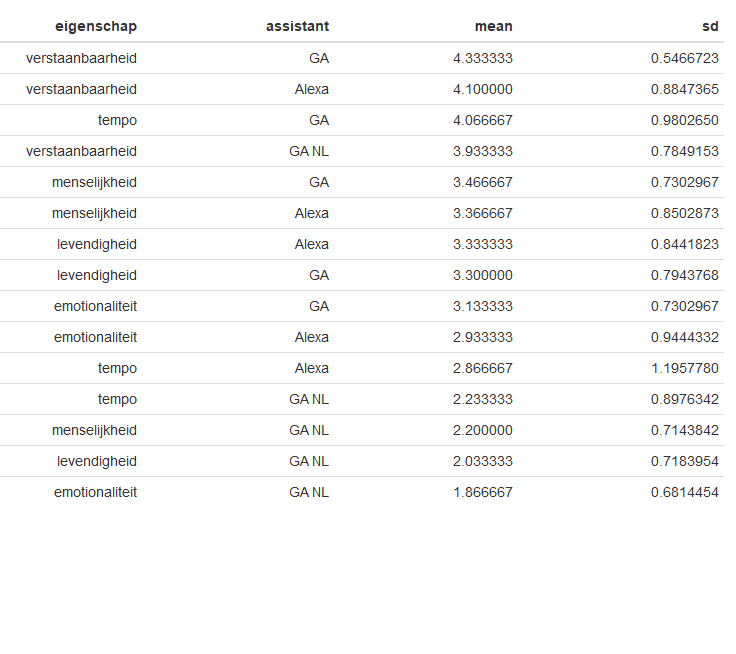
\includegraphics[width=0.9\linewidth]{../onderzoek/onderzoeksresultaten/vergelijking_assistenten_per_eigenschap/table_mean_sd_scores}
    \caption{De gemiddelde scores en standaardafwijkinge van alle assistenten hun eigenschappen gesorteerd van hoog naar laag.}
    \label{fig:table-mean-sd-scores}
\end{figure}

Bij elke eigenschap is te zien hoe \gls{GA NL} lager scoort dan \gls{GA} en Alexa. Zelfs bij verstaanbaarheid, ondanks dat het Nederlands de moedertaal is van elke deelnemer. Het kan wel verklaren waarom het verschil in score tussen \gls{GA NL} aan de ene kant en \gls{GA} en Alexa aan de andere kant bij deze eigenschap het kleinste is. \gls{GA} en Alexa, die beiden in het Engels opereren, scoren gelijkmatig op alle eigenschappen, behalve het tempo. Daar ligt het verschil tussen de drie assistent verdeeld en komt \gls{GA} naar voren als de assistent met de hoogste score.
Twintig van de dertig deelnemers geven aan dat \gls{GA NL} eerder klinkt als een robot, terwijl de helft vindt dat \gls{GA} eerder klinkt als een mens. Ook al gaat het over dezelfde assistent, een verschil in taal zorgt voor heel wat kwaliteitsvermindering.
Emotionaliteit werd als enige eigenschap voor geen enkele assistent beoordeeld met de hoogste score. De verstaanbaarheid is de eigenschap met algemeen de hoogste score.
Levendigheid scoort hoog bij \gls{GA} en Alexa, 25 van de 30 deelnemers gaven voor beide assistenten een score van 3 of meer.

Uit de waarnemingen van de staafdiagrammen en boxplots zijn enkele stellingen geschreven. Voor elke stelling is een t-test uitgevoerd om te bewijzen dat deze statistisch verantwoord of significant zijn. De p-waarde ligt bij elke test duidelijk onder het significantieniveau van 0.05, dus kunnen we steeds de nulhypothese verwerpen. De volgende stellingen zijn bewezen.
\begin{itemize}
    \item Alexa scoort hoger op emotionaliteit dan \gls{GA NL}.
    \item \gls{GA} scoort hoger op emotionaliteit dan \gls{GA NL}.
    \item Alexa scoort hoger op levendigheid dan \gls{GA NL}.
    \item \gls{GA} scoort hoger op levendigheid dan \gls{GA NL}.
    \item Alexa scoort hoger op menselijkheid dan \gls{GA NL}.
    \item \gls{GA} scoort hoger op menselijkheid dan \gls{GA NL}.
    \item \gls{GA} scoort hoger op tempo dan Alexa.
    \item Alexa scoort hoger op tempo dan \gls{GA NL}.
    \item \gls{GA} scoort hoger op verstaanbaarheid dan \gls{GA NL}.
\end{itemize}
Waarom de Nederlandse versie zo verschilt in kwaliteit valt nog verder te onderzoeken.

De resultaten van de uitgevoerde t-testen zijn te vinden onder de map onderzoek/onderzoeksresultaten in de repository beschreven in \ref{s:verwijzing naar repository}.

\subsection{Vergelijking van de eigenschappen per assistent}
\begin{figure}[H]
    \centering
    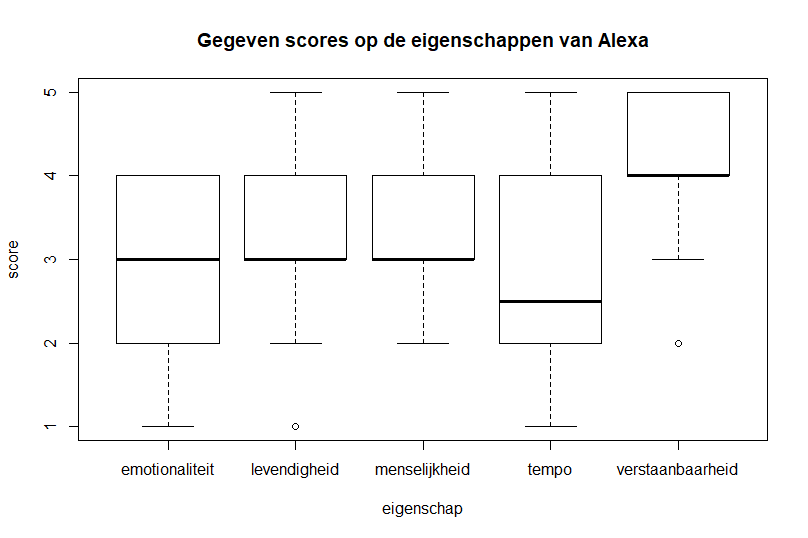
\includegraphics[width=0.9\linewidth]{../onderzoek/onderzoeksresultaten/vergelijking_eigenschappen_per_assistent/boxplot_score_eigenschappen_alexa}
    \caption{De scores die de deelnemers hebben gegeven op de eigenschappen van Alexa}
    \label{fig:boxplot-alexa}
\end{figure}

\begin{figure}[H]
    \centering
    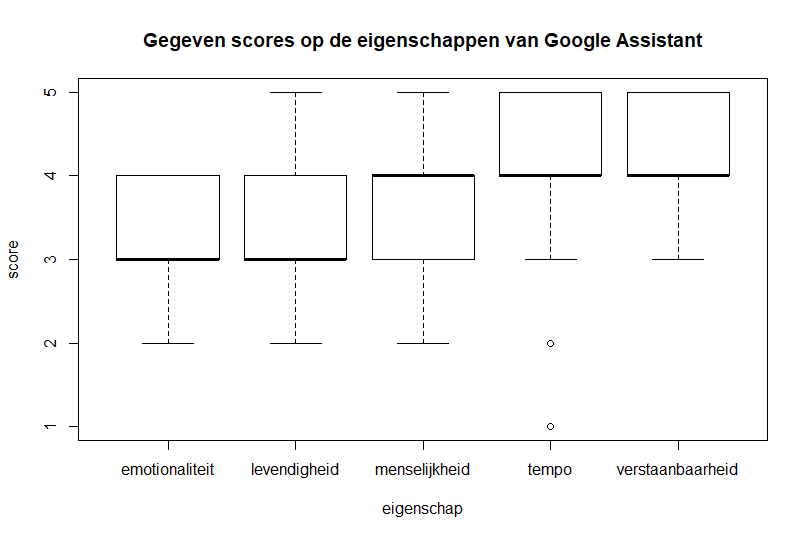
\includegraphics[width=0.9\linewidth]{../onderzoek/onderzoeksresultaten/vergelijking_eigenschappen_per_assistent/boxplot_score_eigenschappen_GA}
    \caption{De scores die de deelnemers hebben gegeven op de eigenschappen van Google Assistant}
    \label{fig:boxplot-ga}
\end{figure}

\begin{figure}[H]
    \centering
    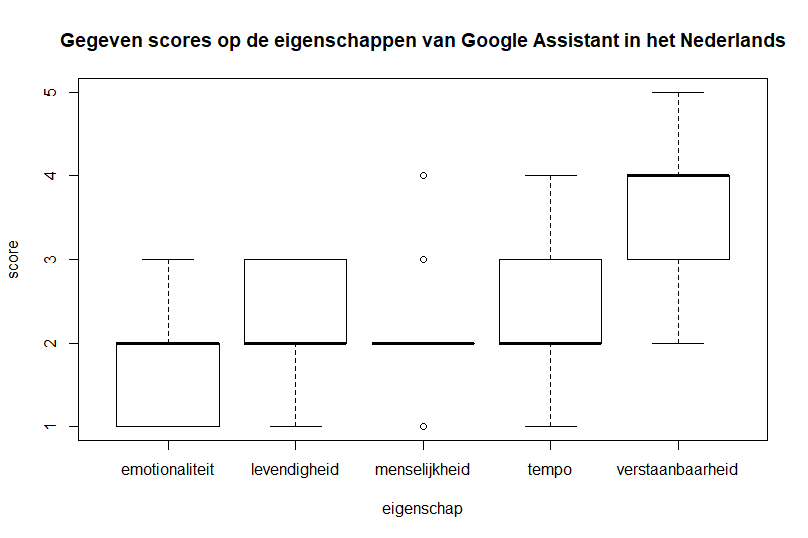
\includegraphics[width=0.9\linewidth]{../onderzoek/onderzoeksresultaten/vergelijking_eigenschappen_per_assistent/boxplot_score_eigenschappen_GA_NL}
    \caption{De scores die de deelnemers hebben gegeven op de eigenschappen van de Nederlandse Google Assistant}
    \label{fig:boxplot-ganl}
\end{figure}

Door de gegeven boxplots kunnen we het onderlinge verschil tussen de eigenschappen van een assistent gaan bekijken. Alexa scoort van alle vijf de eigenschappen het laagst op tempo. Bij \gls{GA} daarentegen hoort het tempo tot één van de betere eigenschappen. De gegeven scores voor het tempo van Alexa zijn het meest verspreid. 
Verstaanbaarheid scoort zowel bij Alexa als bij \gls{GA} steeds een drie of hoger, op één uitschieter na.
\gls{GA} krijgt voor geen enkele eigenschap de laagste score, op één uitschieter na.
\gls{GA NL} scoort op emotionaliteit, levendigheid en menselijkheid nooit hoger dan een 2 of een 3, op 2 uitschieters na.

\section{Vergelijking van de assistenten in spraakherkenning}
\subsection{Een moeilijk te voeren onderzoek}
\label{ss:een moeilijk te voeren onderzoek}
Alexa is er niet in geslaagd om de vraag 'someone fainted and now he is not breathing anymore' ook maar één keer volledig te herkennen door naar de audiofragmenten te luisteren. Google Assistant is hier drie keer in geslaagd. Als de onderzoeker ter controle dezelfde vraag drie keer rechtstreeks stelt aan de assistenten, dan slagen ze er in om minstens 2 van de 3 keren de vraag volledig juist om te vormen naar tekst. Zo kan de opmerking gemaakt worden dat de assistenten slechter scoren op de opgenomen fragmenten dan op een vraag die rechtstreeks wordt gesteld. Hier is echter geen statistisch correct onderzoek naar gedaan.

Een andere bemerking bij het onderzoek is dat elke fout gelijk meetelt. Stel dat twee assistenten de uitspraak 'help me with a burn' omvormen naar tekst. De ene assistent begrijpt de vraag als 'help us for a burn' en de andere als 'tell me with a good'. Het voelt aan alsof de eerste assistent de vraag beter heeft begrepen dan de tweede, terwijl ze toch beide even veel fouten hebben gemaakt. de eerste assistent mist de woorden 'me' en 'with', de tweede assistent de woorden 'help' en 'burn'. Om de correctheid van een gevormde zin beter te interpreteren zou aan elk woord een soort hoofdzakelijkheid voor het begrijpen van de zin moeten toegekend worden. 'help' en 'burn' zijn sleutelwoorden om de zin te begrijpen. Er bestaan echter geen vaste regels om dit aan woorden toe te wijzen.

Als de onderzoeker merkt dat twee woorden verkeerd zijn omgevormd naar één woord, dan geldt de uitzondering dat dit telt als één fout. Een voorbeeld is 'for a whole day' dat wordt herkend door de assistent als 'for all day'. Deze interpretatie is echter niet objectief, waardoor de meting van het aantal fouten nog minder statistisch verantwoord is.

Ondanks dat er verschillende maatregelen zijn genomen om ervoor te zorgen dat elke assistent identiek dezelfde vraag krijgt, is deze opzet toch niet helemaal geslaagd. Alexa neemt elke conversatie op en bewaart ze in uw geschiedenis. Door enkele conversaties van tijdens het onderzoek te beluisteren is er opgemerkt dat hier en daar gekraak aanwezig is. Het gekraak was tijdens het onderzoek niet hoorbaar, waardoor de oorzaak waarschijnlijk bij de microfoon van de smartphone ligt. Het onderzoek is niet correct gevoerd omdat de sterkte van het gekraak kan variëren en mogelijks invloed heeft op de prestaties van de SST van een assistent. Een voorbeeld van een opgenomen interactie met Alexa, inclusief hoorbaar is te vinden onder onderzoek/onderzoeksresultaten/voorbeeld\_opgenomen\_vraag\_alexa in de repository beschreven in \ref{s:verwijzing naar repository}.
De onderzoeker heeft ook waargenomen dat de assistent bij het meermaals luisteren naar hetzelfde audiofragment steeds andere woorden heeft begrepen. Hier zijn geen geschreven resultaten van, maar bevestigen wel nog eens dat de beluisterde commando's variabel zijn.

Door de gegeven redenen is daarom beslist het aantal fouten tussen de assistenten niet te vergelijken. Uit de gevormde zinnen van de assistenten zijn wel enkele andere zaken vastgesteld.

\subsection{De gevormde zinnen}
\begin{figure}[H]
    \centering
    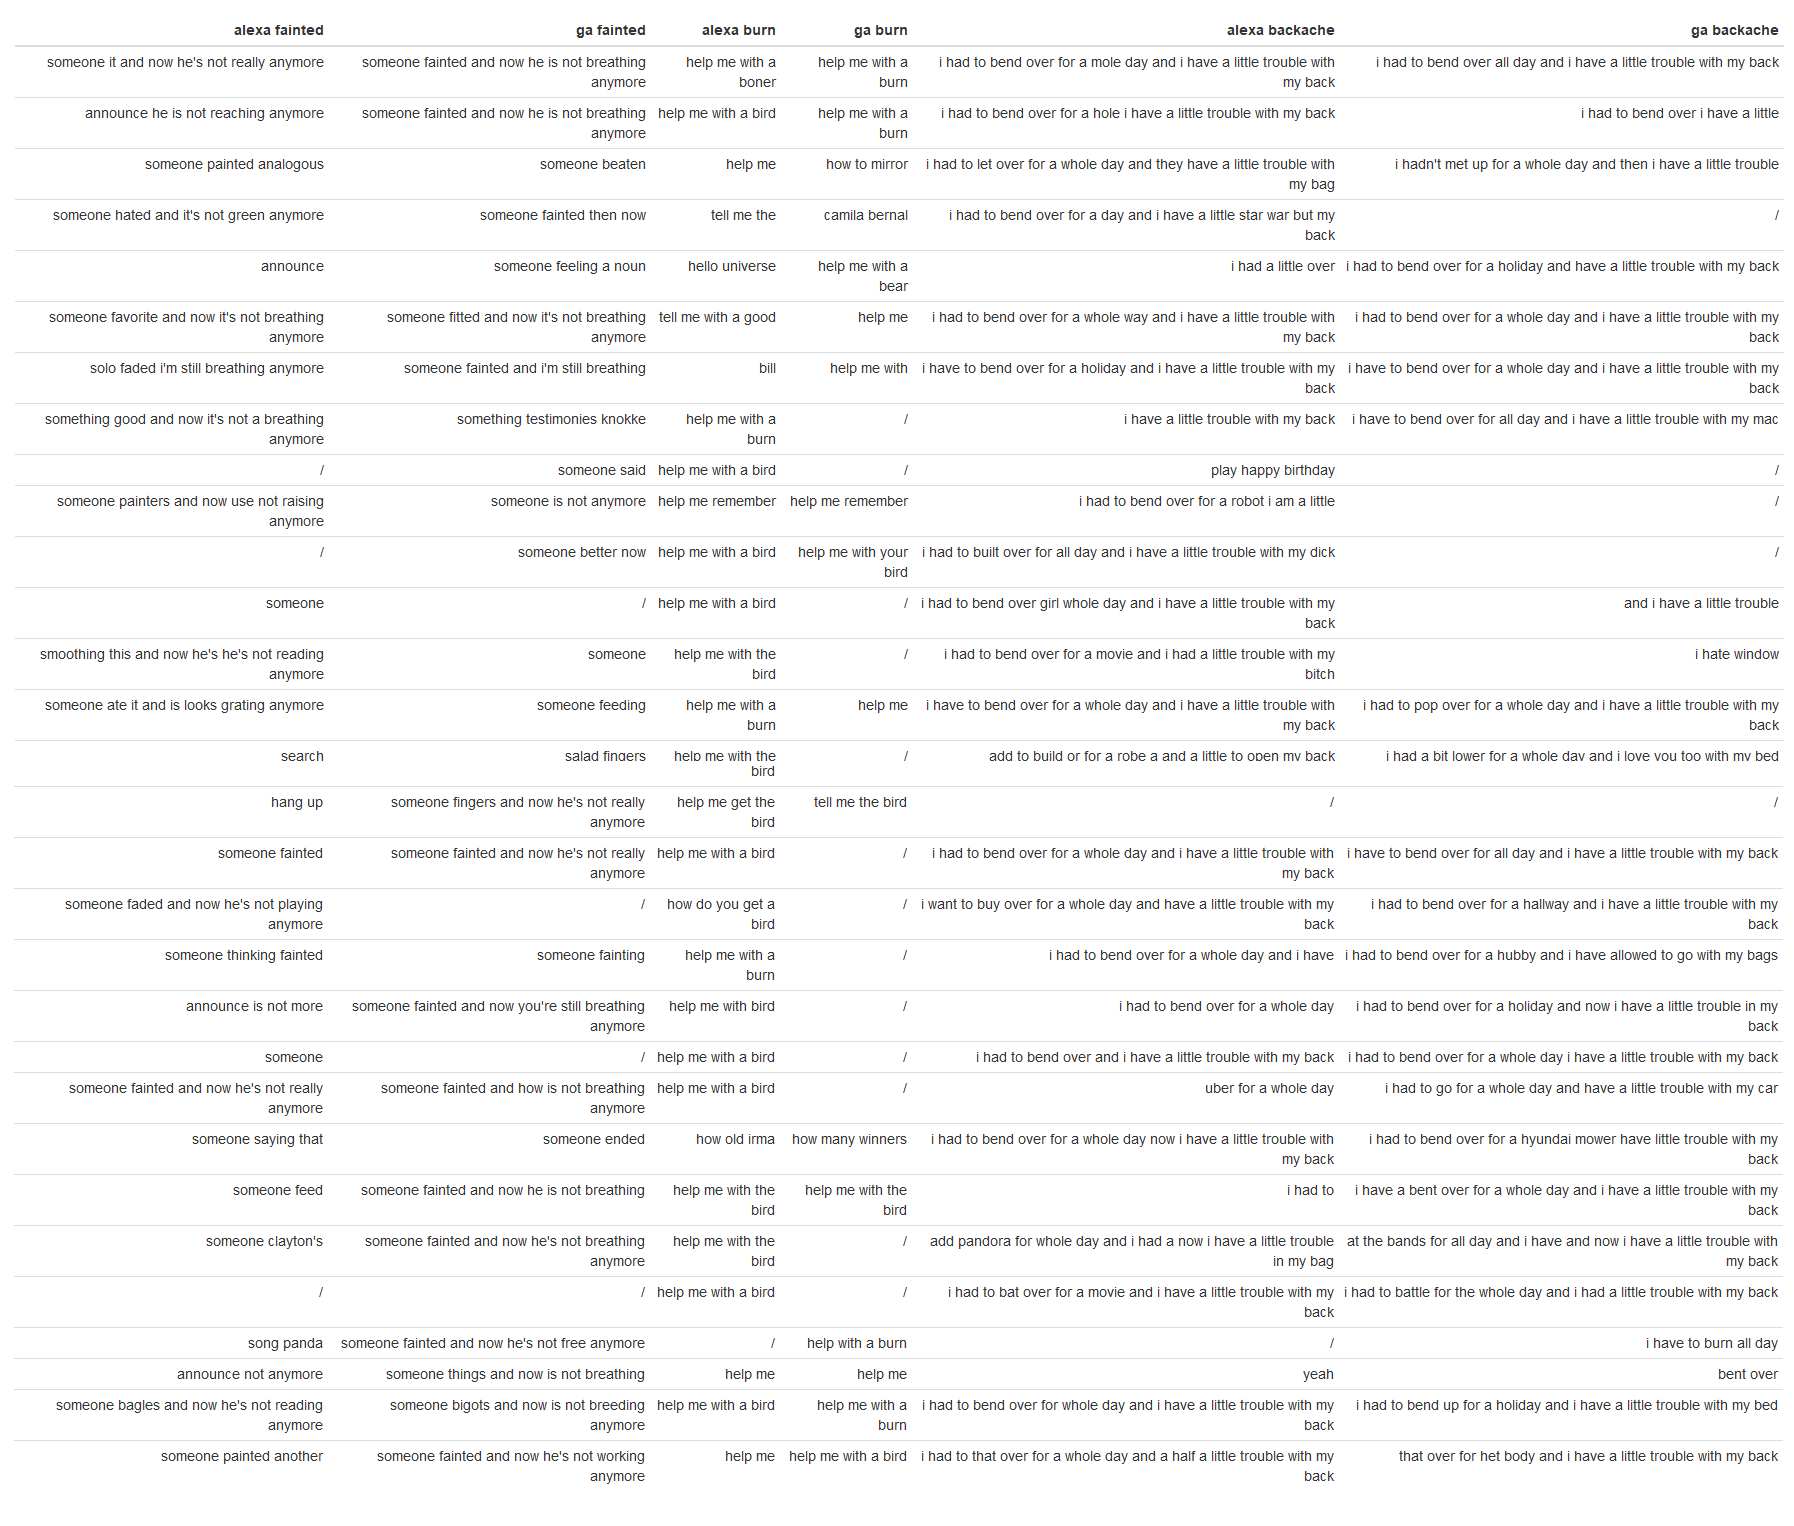
\includegraphics[width=1\linewidth]{../onderzoek/onderzoeksresultaten/vergelijking_tts_alle_teksten/tabel_alle_teksten}
    \caption{Een overzicht van de zinnen die de assistenten hebben begrepen uit de vragen van de deelnemers.}
    \label{fig:tabel-alle-teksten}
\end{figure}

Sommige opvallende zinnen uit de tabel zijn verder onderzocht. Veel woorden zijn geïnterpreteerd als een ander woord dat vergelijkbaar klinkt. De assistenten tonen zowel verschillen als gelijkenissen in het maken van fouten. Enkele voorbeelden zijn:
\begin{itemize}
    \item and now he's-> announce
    \item burn -> bird, bear
    \item fainted -> faded, fingers, favorite, hated, ate, painted
    \item whole -> mole, all, hole
    \item whole day -> holiday
    \item breathing -> breeding, reaching
\end{itemize}
Waar de assistenten het dus nog steeds moeilijk mee hebben is het onderscheiden van woorden die gelijke klanken vertonen.

In \ref{s:spraakgestuurde technologie} is te lezen hoe een model beslist welke woorden te vormen door onder meer de waarschijnlijkheid dat een bepaald woord na een ander komt. Google Assistant en Alexa hebben beide volgende fout gemaakt in de reeks: 'Someone fainted and now he is not really anymore'. Drie keren werd er beslist om van de uitspraak waar 'not breathing' wordt uitgesproken, 'not really' te maken. 'Not really' is een combinatie die vaak kan voorkomen omdat het kan gebruikt als negatie wanneer de assistent iets vraagt.

In \ref{s:de geschiedenis van spraakassistenten} wordt meer verteld over hoe praten met een spraakassistent nooit echt als een conversatie aanvoelde doordat de gebruiker voor een lange tijd verplicht werd een pauze te laten tussen elk woord. Met de technologie die we vandaag hebben is dit niet meer van toepassing, maar toch worden nog fouten gemaakt door het vlot uitspreken van meerdere woorden na elkaar. Deze fout is er een voorbeeld van. 'And now he is' werd herkend als 'announce'. Als je 'and now he is' snel uitspreekt, kan je merken dat dit inderdaad iets weg heeft van het woord 'announce'.
%%=============================================================================
%% De eerste hulp assistent
%%=============================================================================

\chapter{De eerste hulp assistent}
\label{ch:De eerste hulp assistent}

\section{De functionaliteiten}
\label{De functionaliteiten}

\section{Persona}
\label{Persona}




% Voeg hier je eigen hoofdstukken toe die de ``corpus'' van je bachelorproef
% vormen. De structuur en titels hangen af van je eigen onderzoek. Je kan bv.
% elke fase in je onderzoek in een apart hoofdstuk bespreken.

%\input{...}
%\input{...}
%...

%%=============================================================================
%% Conclusie
%%=============================================================================

\chapter{Conclusie}
\label{ch:conclusie}

%% TODO: Trek een duidelijke conclusie, in de vorm van een antwoord op de
%% onderzoeksvra(a)g(en). Wat was jouw bijdrage aan het onderzoeksdomein en
%% hoe biedt dit meerwaarde aan het vakgebied/doelgroep? Reflecteer kritisch
%% over het resultaat. Had je deze uitkomst verwacht? Zijn er zaken die nog
%% niet duidelijk zijn? Heeft het onderzoek geleid tot nieuwe vragen die
%% uitnodigen tot verder onderzoek?

\lipsum[76-80]



%%=============================================================================
%% Bijlagen
%%=============================================================================

\appendix

%%---------- Onderzoeksvoorstel -----------------------------------------------

\chapter{Onderzoeksvoorstel}

Het onderwerp van deze bachelorproef is gebaseerd op een onderzoeksvoorstel dat vooraf werd beoordeeld door de promotor. Dat voorstel is opgenomen in deze bijlage.

% Verwijzing naar het bestand met de inhoud van het onderzoeksvoorstel
%---------- Inleiding ---------------------------------------------------------

\section{Introductie} % The \section*{} command stops section numbering
\label{sec:introductie}

Hier introduceer je werk. Je hoeft hier nog niet te technisch te gaan.

Je beschrijft zeker:

\begin{itemize}
  \item de probleemstelling en context
  \item de motivatie en relevantie voor het onderzoek
  \item de doelstelling en onderzoeksvraag/-vragen
\end{itemize}

%---------- Stand van zaken ---------------------------------------------------

\section{State-of-the-art}
\label{sec:state-of-the-art}

Hier beschrijf je de \emph{state-of-the-art} rondom je gekozen onderzoeksdomein. Dit kan bijvoorbeeld een literatuurstudie zijn. Je mag de titel van deze sectie ook aanpassen (literatuurstudie, stand van zaken, enz.). Zijn er al gelijkaardige onderzoeken gevoerd? Wat concluderen ze? Wat is het verschil met jouw onderzoek? Wat is de relevantie met jouw onderzoek?

Verwijs bij elke introductie van een term of bewering over het domein naar de vakliteratuur, bijvoorbeeld~\autocite{Doll1954}! Denk zeker goed na welke werken je refereert en waarom.

% Voor literatuurverwijzingen zijn er twee belangrijke commando's:
% \autocite{KEY} => (Auteur, jaartal) Gebruik dit als de naam van de auteur
%   geen onderdeel is van de zin.
% \textcite{KEY} => Auteur (jaartal)  Gebruik dit als de auteursnaam wel een
%   functie heeft in de zin (bv. ``Uit onderzoek door Doll & Hill (1954) bleek
%   ...'')

Je mag gerust gebruik maken van subsecties in dit onderdeel.

%---------- Methodologie ------------------------------------------------------
\section{Methodologie}
\label{sec:methodologie}

Hier beschrijf je hoe je van plan bent het onderzoek te voeren. Welke onderzoekstechniek ga je toepassen om elk van je onderzoeksvragen te beantwoorden? Gebruik je hiervoor experimenten, vragenlijsten, simulaties? Je beschrijft ook al welke tools je denkt hiervoor te gebruiken of te ontwikkelen.

%---------- Verwachte resultaten ----------------------------------------------
\section{Verwachte resultaten}
\label{sec:verwachte_resultaten}

Hier beschrijf je welke resultaten je verwacht. Als je metingen en simulaties uitvoert, kan je hier al mock-ups maken van de grafieken samen met de verwachte conclusies. Benoem zeker al je assen en de stukken van de grafiek die je gaat gebruiken. Dit zorgt ervoor dat je concreet weet hoe je je data gaat moeten structureren.

%---------- Verwachte conclusies ----------------------------------------------
\section{Verwachte conclusies}
\label{sec:verwachte_conclusies}

Hier beschrijf je wat je verwacht uit je onderzoek, met de motivatie waarom. Het is \textbf{niet} erg indien uit je onderzoek andere resultaten en conclusies vloeien dan dat je hier beschrijft: het is dan juist interessant om te onderzoeken waarom jouw hypothesen niet overeenkomen met de resultaten.



%%---------- Andere bijlagen --------------------------------------------------
% TODO: Voeg hier eventuele andere bijlagen toe
%\input{...}

%%---------- Referentielijst --------------------------------------------------
\printbibliography[heading=bibintoc]
%\addcontentsline{toc}{chapter}{\textcolor{maincolor}{\IfLanguageName{dutch}{Bibliografie}{Bibliography}}}

\end{document}
